\documentclass[11.5pt]{article}
\usepackage[utf8]{inputenc}
\usepackage[T1]{fontenc}
\usepackage[textwidth = 460pt,top = 80pt, bottom = 80pt]{geometry}
\usepackage{graphicx}
\usepackage[justification=default]{subfig} %Manage sub-figures 
\usepackage[update]{epstopdf}
\usepackage[labelfont=bf]{caption}
\usepackage[dvipsnames]{xcolor}
\usepackage{fancyhdr}
\usepackage{amsmath}
\usepackage{booktabs}
\usepackage{mathabx}
\usepackage{multicol}
\usepackage{multirow}
\usepackage{mcode}
\usepackage{titling}
\usepackage{amssymb}
\usepackage{mathabx}
\usepackage{bm}
\usepackage[leqno,fleqn,intlimits]{empheq}

%Fonts
%\usepackage{librebaskerville}
%\usepackage{arev}
%\usepackage{concmath}
%\usepackage[lf]{Baskervaldx}
%\usepackage{librecaslon}
%\usepackage{gfsartemisia-euler}
%\usepackage[urw-garamond]{mathdesign}
%\usepackage{mlmodern}


%Bibliography

\usepackage{csquotes}
\usepackage[sorting=none,%
sortcites=true,%
bibencoding=ascii,%
autopunct=true,%
hyperref=true,%
language=auto,%
%backref=true,%
url=false,%
%maxcitenames=10,%
%minbibnames = 20,%
maxbibnames = 3,%
giveninits, 
natbib = false,
isbn=false,%
backend=biber]{biblatex}
\addbibresource{bibliography.bib}

%Headers and footers
\pagestyle{fancy}
\fancyhf{}
\rhead{SADC: final project}
\lhead{Lorenzo Porcelli 945295}
\rfoot{\thepage}
\lfoot{AY 2020-21 -- Prof. F. Bernelli Zazzera, T.A. A. Colagrossi}
\renewcommand{\headrulewidth}{1.5pt}
\renewcommand{\footrulewidth}{1.5pt}


\fancypagestyle{empty}{         
    \fancyhf{}  
    \renewcommand{\headrulewidth}{0pt}
    \renewcommand{\footrulewidth}{0pt}
}

\usepackage[]{hyperref}
\usepackage{cleveref}
%%% CREF setup
\crefname{equation}{Eq.}{Eqs.}
\crefname{table}{Table}{Tables}
\crefname{figure}{Fig.}{Figs.}


\begin{document}

\begin{titlingpage}
\begin{center}
    \begin{figure}
        \centering
        
\includegraphics[width=0.6\textwidth]{graphics/logopolimi_mod.jpg}
    \end{figure}
\Large{\textsc{Politecnico di Milano \\ Department of Aerospace Science and Technology (DAER) \\ M.Sc. in Space Engineering}}

\vspace{1cm}

\rule{0.95\textwidth}{0.7mm}
{\Large{\textbf{Final project: \\Design and simulation of an ADCS system for a 6U CubeSat}}}
\rule{0.95\textwidth}{0.7mm}

\vspace{1cm}

\large{\textbf{Spacecraft Attitude Dynamics and Control}}

\large{Prof. Franco Bernelli Zazzera \\ A.Y. 2020-2021}

\vspace{1cm}

Lorenzo Porcelli, mat. 945295

\end{center}

\end{titlingpage}

\pagenumbering{roman}

\tableofcontents

\clearpage

\setcounter{page}{1}
\pagenumbering{arabic}

\section{Introduction} \label{sec:introduction}

The aim of the project is to develop an attitude determination and control system for a 6U CubeSat in the LEO environment using COTS products. The following report presents the modeling of the dynamics of the spacecraft, the design of the ADCS system and finally the results of numerical simulations.

The spacecraft is modeled taking inspiration from \textit{RainCube} (\textbf{Ra}dar \textbf{in} a \textbf{Cube}Sat \cite{raincube}), which was an Earth observation satellite carrying a Nadir pointing antenna for radar measurements. The spacecraft was launched in 2018 and eventually decayed in December 2020. The considered mission profile will be divided in three phases:

\begin{enumerate}
    \item an \textbf{uncontrolled} phase, right after orbit insertion
    \item a \textbf{de-tumbling} phase
    \item a \textbf{tracking} phase, in which the spacecraft is constantly re-oriented for mission purposes
\end{enumerate}


\section{Description of the system}

\subsection{Configuration and inertia properties of the spacecraft}

The model used for the satellite structure is depicted in \cref{fig:cubesat}. The central body consists of two rows of 3U blocks, where U = $0.1 \,m$. Two 3U x 2U solar panels are attached to the top side of the main structure. The mass and the dimensions of these components are reported in \cref{tab:mass_dimensions}.

\begin{figure}[h]
    \centering
    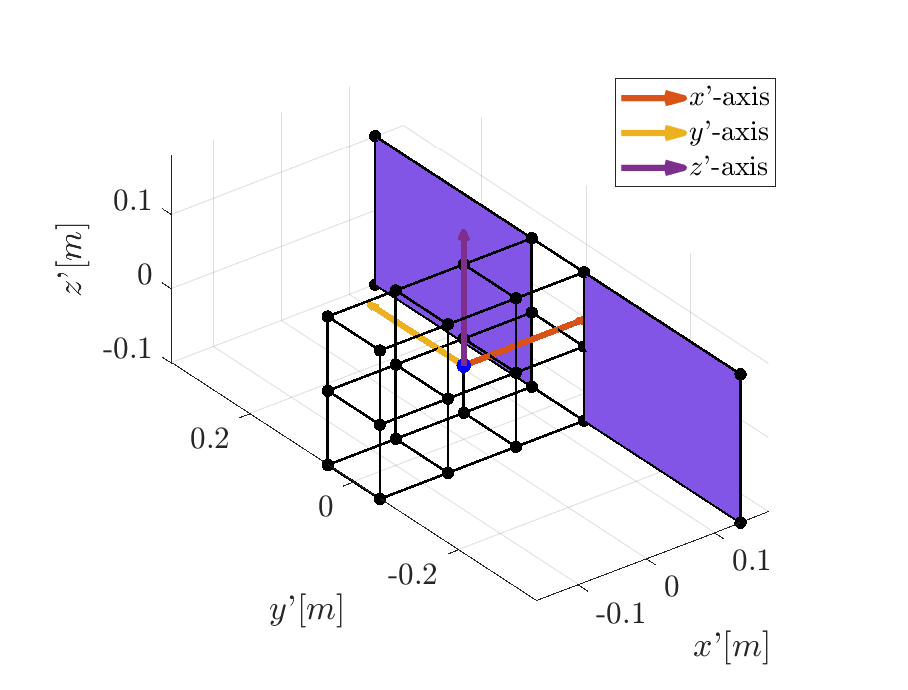
\includegraphics[width=0.7\textwidth]{graphics/cubesat.eps}
    \caption{Graphical representation of the 6U CubeSat}
    \label{fig:cubesat}
\end{figure}

\begin{table}[h]
    \centering
    \caption{Mass and dimensions of the satellite parts}
    \begin{tabular}{lcc}
    \toprule
    \toprule
    \textbf{Components} & \textbf{Mass} & \textbf{Dimensions} \\
    \midrule
    Main body & 6x 1 $kg$ & 0.3 x 0.2 x 0.1 $m$ \\
    \midrule
    Two solar panels & 2x 0.25 $kg$ & (2x) 0.3 x 0.2 x 0.005 $m$ \\
    \bottomrule
    \bottomrule
    \end{tabular}
    \label{tab:mass_dimensions}
\end{table}

\cref{fig:cubesat} also reports the frame of reference \{$x'$, $y'$, $z'$\}, placed in the geometrical centre of the satellite. In this frame of reference, the centre of gravity of the satellite has coordinates: $$ \mathbf{r}'_{CG} = \begin{bmatrix} 0.013 & 0 & 0 \end{bmatrix}^T\, m $$ These axes are parallel to the principal axes of inertia, which will be referred to as \{$x$, $y$, $z$\} (or body frame).

Considering the mass properties of the spacecraft and the dimensions of the components, the inertia matrix (referred to the CG in the principal axes) is equal to:

$$ I = \begin{bmatrix} 0.0504 & 0 & 0 \\
0 & 0.0771 & 0 \\
0 & 0 & 0.0841 
\end{bmatrix} kg \cdot m^2 $$

\subsection{Sensors}

The spacecraft is equipped with a Sun sensor, a star tracker and a magnetometer. The first two are used to generate measurements of the directions of celestial bodies, while the last one is sensible to Earth's magnetic field.

\subsubsection{Sun sensor}

The selected Sun sensor is the two-axis \textit{SSOC-D60} sensor, produced by \textit{SolarMems}. Its specifications are reported in \cref{tab:sun_sensor}.

\begin{table}[h]
    \centering
    \caption{SSOC-D60 specifications \cite{sun_sensor}}
    \begin{tabular}{cccccc}
    \toprule
    \toprule
    \textbf{Dimensions} & \textbf{Mass} & \textbf{FoV} & \textbf{Max. update rate} & \textbf{Accuracy} \\
    \midrule
    30 x 60 x 12 $mm$ & 35 $g$ & 120$^{\circ}$ ($\pm$60$^{\circ}$) & 50 $Hz$ & < 0.3$^{\circ}$ \\
    \bottomrule
    \bottomrule
    \end{tabular}
    \label{tab:sun_sensor}
\end{table}

The field of view is assumed to be conical. The sensor is placed on the top side of the spacecraft, next to the solar panels, so its coordinates in the \{$x'$, $y'$, $z'$\} frame are $\mathbf{r}'_{SS} = [0.15,\, 0,\, 0]^T \, m$. The sensor frame is aligned with the principal axes, so the rotation matrix from the body frame to the sensor frame $A_{s/b}^{SS}$ is simply the identity matrix $\mathbb{I}_3$

\subsubsection{Star tracker}

The chosen star tracker is \textit{arcsec}'s \textit{Sagitta}, whose specifications are reported in \cref{tab:star_tracker}. It can track up to 32 stars simultaneously and up to magnitude 6.

\begin{table}[h]
    \centering
    \caption{Sagitta specifications \cite{star_tracker}}
    \begin{tabular}{cccccc}
    \toprule
    \toprule
    \textbf{Dimensions} & \textbf{Mass} & \textbf{FoV} & \textbf{Max. update rate} & \multicolumn{2}{c}{\textbf{Accuracy}} \\
    \midrule
    \multirow{2}{*}{44 x 50 x 95 $mm$} & \multirow{2}{*}{250 $g$} & \multirow{2}{*}{40$^{\circ}$ ($\pm$20$^{\circ}$)} & \multirow{2}{*}{5 $Hz$} & cross-bore s. & roll-bore s. \\
    \cmidrule{5-6}
    & & & & 2" & 10"  \\
    \bottomrule
    \bottomrule
    \end{tabular}
    \label{tab:star_tracker}
\end{table}

The field of view is assumed to be conical. The position of the sensor in the \{$x'$, $y'$, $z'$\} frame is $\mathbf{r}'_{ST} = [-0.1,\, 0.05,\, 0]^T \,m$. The bore sight direction (considered to be the $1^{st}$ axis in the sensor frame) is coincident with the $y$-axis of the body frame, while the $3^{rd}$ axis is directed as $z$. The rotation matrix from the body frame to the sensor frame is therefore:

$$ A_{s/b}^{ST} = \begin{bmatrix}
0 & 1 & 0 \\
-1 & 0 & 0 \\
0 & 0 & 1
\end{bmatrix} $$

\subsubsection{Magnetometer}

The specifications of the selected magnetometer, \textit{NSS Magnetometer} by \textit{New Space Systems}, are presented in \cref{tab:magnetometer}. The sensor provides tri-axial measurements of the magnetic field.

\begin{table}[h]
    \centering
    \caption {NSS Magnetometer specifications \cite{magnetometer}}
    \begin{tabular}{ccccc}
    \toprule
    \toprule
    \textbf{Dimensions} & \textbf{Mass} & \textbf{Max. update rate} & \textbf{Noise density @} 1 $Hz$ & \textbf{Orthogonality} \\
    \midrule
    99 x 43 x 17 $mm$ & 85 $g$ & 18 $Hz$ & 16 $nT$ $rms/Hz$ & $\leq 1^{\circ}$ \\
    \bottomrule
    \bottomrule
    \end{tabular}
    \label{tab:magnetometer}
\end{table}

\subsection{Actuators}

The spacecraft is equipped with a magnetorquer and a set of four reaction wheels.

\subsubsection{Magnetorquer}

The chosen magnetorquer is the \textit{NanoTorque GST-600}, developed by \textit{GomSpace}. It is composed of three coils which generate magnetic dipoles in three orthogonal directions (which are, in this case, coincident with the axes of the body frame). Its properties are reported in \cref{tab:magnetorquer}.

\begin{table}[h]
    \centering
    \caption{GST-600 specifications \cite{magnetorquer}}
    \begin{tabular}{cccc}
    \toprule
    \toprule
    \multirow{2}{*}{\textbf{Dimensions}} & \multirow{2}{*}{\textbf{Mass}} & \textbf{Max. dipole strength} & \textbf{Max. dipole strength} \\
    & & ($x-$, $y-$axis) & ($z-$axis) \\
    \midrule
    90.5 x 96.9 x 17.2 $mm$ & 156 $g$ & 0.31 $A/m^2$ & 0.34 $A/m^2$ \\
    \bottomrule
    \bottomrule
    \end{tabular}
    \label{tab:magnetorquer}
\end{table}

\subsubsection{Reaction wheels}

The selected set of reaction wheels is the \textit{SatBus 4RW0} by \textit{NanoAvionics}. It consists of four identical wheels arranged in a pyramid configuration. The specifications of this product are reported in \cref{tab:reaction_wheels}.

\begin{table}[h]
    \centering
    \caption{SatBus 4RW0 specifications}
    \begin{tabular}{ccccc}
    \toprule
    \toprule
    \multirow{2}{*}{\textbf{Dimensions}} & \multirow{2}{*}{\textbf{Mass}} & \textbf{Inertia moment around} & \textbf{Max. torque} & \textbf{Max. momentum} \\
    & & \textbf{spin axis} (single wheel) & (single wheel) &  (single wheel) \\
    \midrule
    92.5 x 92.5 x 51.3 $mm$ & 665 $g$ & 3.24 $\cdot 10^{-5}\,kg\cdot m^2$ & 3.2 $mN \cdot m$ & $20 \, mN \cdot ms$ \\
    \bottomrule
    \bottomrule
    \end{tabular}
    \label{tab:reaction_wheels}
\end{table}

\section{Description of the model}

\subsection{Orbital dynamics}

The orbital dynamics of the satellite is modeled as an unperturbed two body problem, considering the Earth as the primary body. The perturbations are included only in the rotational dynamics of the spacecraft. The reference orbit is taken from the last update for RainCube's TLE \cite{raincube_orbit}, whose first five Keplerian elements were:

\begin{table}[h!]
    \centering
    \caption{Keplerian elements of the orbit}
    \begin{tabular}{ccccc}
    \toprule
    \toprule
    \textbf{Semi-major axis} $a$ & \textbf{Eccentricity} $e$ & \textbf{Inclination} $i$ & \textbf{RAAN} $\Omega$ & \textbf{Argument of perigee} $\omega$ \\
    \midrule
    6779.4 km &  1.98 $\cdot10^{-4}$ & 51.6$^{\circ}$ & 23.4$^{\circ}$ & 43.9$^{\circ}$ \\
    \bottomrule
    \bottomrule
    \end{tabular}
    \label{tab:keplerian_elements}
\end{table}

As the dynamics is unperturbed, the only varying element is the true anomaly $\theta$, whose evolution in time is given by the equation:

\begin{equation}
    \dot{\theta} = \sqrt{\frac{\mu_{\Earth}}{a^3}} \frac{(1 + e\,\cos \theta)^2}{(1 - e^2)^{3/2}}
\end{equation}

where $\mu_{\Earth}$ is the gravitational parameter of the Earth, equal to $398600\,km^3/s^2$. The integration of the true anomaly allows for the computation of the position and the velocity of the spacecraft in the Earth Centered Inertial (\textit{ECI}) frame (respectively $\mathbf{r}_{S/C}$ and $\mathbf{v}_{S/C}$) at any time. These vectors are required in order to derive the disturbing torques acting on the spacecraft. The variation of the true anomaly also entails the time variation of the rotation matrix from the Local Horizontal Local Vertical (\textit{LVLH}) frame to the inertial frame $A_{l/n}$ (\cref{eq:A_ln}). This element is necessary for the design of the control in the tracking phase. Uncertainties on $\mathbf{r}_{S/C}$, $\mathbf{v}_{S/C}$ and $A_{l/n}$ are neglected.

\begin{equation}
    A_{l/n} = \begin{bmatrix} \cos \theta & \sin \theta & 0 \\
    - \sin \theta & \cos \theta & 0 \\
    0 & 0 & 1
    \end{bmatrix}
    \begin{bmatrix}
    1 & 0 & 0 \\
    0 & \cos i & \sin i \\
    0 & - \sin i & \cos i \\
    \end{bmatrix}
    \label{eq:A_ln}
\end{equation}

The direction of the Sun in the ECI, which will be needed for the simulation of the disturbances and for the Sun sensor, is computed considering the orbit of the Earth as circular (with radius equal to $1 \, AU$):

\begin{equation}
    \hat{\mathbf{R}}_{\Sun,n} = \begin{bmatrix}
    \cos (n_{\Sun} t) \\
    \sin (n_{\Sun} t) \cos \epsilon \\
    \sin (n_{\Sun} t) \sin \epsilon
    \end{bmatrix}
\end{equation}

where $n_{\Sun} = 2 \pi / 1\,year$ is the apparent mean motion of the Sun and $\epsilon = 23.45^{\circ}$ is the obliquity angle.

\subsection{Rotational dynamics and kinematics}

The spacecraft is modeled as a rigid body, so its rotational dynamics can be described through Euler's equations:

\begin{equation}
    I \frac{\mathrm{d} \bm{\omega}}{\mathrm{d} t} = I \bm{\omega} \times \bm{\omega} + \mathbf{M}_d + \mathbf{M}_c
    \label{eq:euler}
\end{equation}

where $\bm{\omega} = [\omega_x,\, \omega_y,\, \omega_z]^T$ is the angular velocity of the satellite, $\mathbf{M}_d$ is the disturbing torque and $\mathbf{M}_c$ is the control torque. Every quantity is expressed in the satellite's body frame. All the terms contributing to the disturbing torque will be presented in \cref{sec:disturbances}, while the control torque will be the target of the design in \cref{sec:control}. 

The numerical integration of \cref{eq:euler} returns the value of the angular velocity, which can subsequently be used to propagate the attitude kinematics of the satellite. The chosen attitude parameter, which describes the orientation of the body frame with respect to the inertial frame, is the quaternion $q$, whose time evolution is described by the following differential equation:

\begin{equation}
    \dot{q} = \frac{1}{2} \begin{bmatrix}
    0 & \omega_z & - \omega_y & \omega_x \\
    - \omega_z & 0 & \omega_x & \omega_y \\
    \omega_y & - \omega_x & 0 & \omega_z \\
    - \omega_x & - \omega_y & -\omega_z & 0
    \end{bmatrix} q = \frac{1}{2} \Omega q
\end{equation}

$q$ is normalized at each integration step in order to preserve its property of having unitary magnitude. From the knowledge of $q$, the direction cosine matrix (\textit{DCM}) of the body frame is derived as:

\begin{equation}
    A_{b/n} = (q_4 - \mathbf{q}^T \mathbf{q})\,\mathbb{I}_3 + 2 \mathbf{q} \mathbf{q}^T - 2 q_4 [q \wedge]
    \label{eq:dcm}
\end{equation}

$\mathbf{q}$ is the vector part of the quaternion and $q_4$ is its scalar part, such that $q = [\mathbf{q}, \, q_4]^T$. The $[\cdot \wedge]$ symbol stands for the cross product matrix operator.

\subsection{External disturbances} \label{sec:disturbances}

The total disturbing torque $\mathbf{M}_d$ is made up of four contributions: $\mathbf{M}_{\mathbf{b}}$ from the interaction with the magnetic field, $\mathbf{M}_{GG}$ from the gravity gradient, $\mathbf{M}_{drag}$ from atmospheric drag and $\mathbf{M}_{SRP}$ from solar radiation pressure.

\subsubsection{Earth's magnetic field}

The Earth's magnetic field at the spacecraft position is simulated using a simple dipole model, derived from the first order expansion of the spherical harmonic potential.

\begin{equation}
    \mathbf{b}_n = \frac{R_{\Earth}^3 H_0}{\| \mathbf{r}_{S/C} \|^3}\,[3\,(\hat{\mathbf{m}} \cdot \hat{\mathbf{r}}) \, \hat{\mathbf{r}} - \hat{\mathbf{m}}], \text{ where } H_0 = \sqrt{(g_1^0)^2 + (g_1^1)^2 + (h_1^1)^2}
\end{equation}

The term $H_0$ is computed from the first order Gaussian coefficients of the International Geomagnetic Reference Field (\textit{IGRF}) 2000 \cite{igrf}. $R_{\Earth}$ is Earth's equatorial radius (equal to 6378.1 $km$), $\hat{\mathbf{r}}$ is the unit vector in the direction of $\mathbf{r}_{S/C}$, and $\hat{\mathbf{m}}$ is the direction of the magnetic dipole:

\begin{equation}
    \hat{\mathbf{m}} = \begin{bmatrix}
    \sin (11.5^{\circ})\, \cos (\omega_{\Earth} t) \\
    \sin (11.5^{\circ})\, \sin (\omega_{\Earth} t) \\
    \cos (11.5^{\circ})
    \end{bmatrix}
\end{equation}

$\omega_{\Earth}$ is the angular speed of Earth's rotation in inertial space (equal to $7.29 \cdot 10^{-5}\, rad/s$). The torque acting on the satellite can be finally computed as:

\begin{equation}
    \mathbf{M}_{\mathbf{b}} = \mathbf{D}_r \times \mathbf{b}_b = \mathbf{D}_r \times (A_{b/n} \mathbf{b}_n )
\end{equation}

where $\mathbf{D}_r$ is the residual magnetic dipole of the spacecraft, assumed to be $[0.01, \, 0.01, \, 0.01]^T \, A/m^2$.

\subsubsection{Gravity gradient torque}

The torque coming from the non uniform gravity field acting on the spacecraft can be determined as:

\begin{equation}
    \mathbf{M}_{GG} = \frac{3 \mu_{\Earth}}{\| \mathbf{r}_{S/C} \|^3} \begin{bmatrix}
    (I_z - I_y)\, c_2\,c_3 \\
    (I_x - I_z)\, c_1\,c_3 \\
    (I_y - I_x)\, c_1\,c_2
    \end{bmatrix}
    \label{eq:gravity-gradient}
\end{equation}

This expression hold as long as $I$ is a diagonal matrix, such that $I = \text{diag}\,(I_x,\,I_y,\,I_z)$. The terms $c_1,\,c_2,\,c_3$ are computed as:

\begin{equation}
    \begin{bmatrix}
    c_1 \\
    c_2 \\
    c_3 
    \end{bmatrix}
    = A_{l/n} A_{b/n}^T
    \begin{bmatrix}
    1 \\
    0 \\
    0
    \end{bmatrix}
    = A_{b/l}
    \begin{bmatrix}
    1 \\
    0 \\
    0
    \end{bmatrix}
\end{equation}

\subsubsection{Atmospheric drag} \label{sec:drag}

The torque due to the aerodynamic interaction of the satellite with the atmosphere is computed dividing the body into $M$ planar surfaces with area $A_i$, each one identified by its normal unit vector $\hat{\mathbf{n}}_{b,i}$ in the body frame. For each surface $i$, the drag force can be computed as:

\begin{equation}
    \mathbf{F}_{drag,i} = 
    \begin{cases}
    - \frac{1}{2} \rho\,c_D \, A_{i} \, \| \mathbf{v}_{rel,b,i} \|^2 \, \left( \hat{\mathbf{n}}_{b,i} \cdot \frac{\mathbf{v}_{rel,b,i}}{\| \mathbf{v}_{rel,b,i} \|} \right) & \text{if } \hat{\mathbf{n}}_{b,i} \cdot \frac{\mathbf{v}_{rel,b,i}}{\| \mathbf{v}_{rel,b,i} \|} > 0 \\
    0 & \text{otherwise} \\
    \end{cases}
\end{equation}


The velocities in the body frame $\mathbf{v}_{rel,b,i} = A_{b,n}\, \mathbf{v}_{rel,n,i}$ depend on the relative velocity between each surface and the rotating atmosphere in the inertial frame. Using Rivals' theorem:

\begin{equation}
\mathbf{v}_{rel,n,i} = (\mathbf{v}_{S/C} + \bm{\omega} \times \mathbf{r}_{b,i}) - \bm{\omega}_{\Earth} \times \mathbf{r}_{S/C}    
\end{equation}

with $\bm{\omega}_{\Earth}$ being the angular velocity vector of the Earth. The vectors $\mathbf{r}_{b,i}$ represent the positions of the geometrical centres of the surfaces with respect to the centre of gravity of the spacecraft in the body frame. The term due to the rotation of the spacecraft $\bm{\omega} \times \mathbf{r}_{b,i}$ is negligible for low angular velocities, thus it is assumed that the relative velocity of each surface is equal to the one of the centre of gravity, such that $\textbf{v}_{rel,b,i} \approx \mathbf{v}_{rel,b} = \mathbf{v}_{S/C} - \bm{\omega}_{\Earth} \times \mathbf{r}_{S/C}$. The density $\rho$ is considered constant and equal to $3.725 \cdot 10^{-12}\, kg/m^3$, according to the \textit{CIRA72} model \cite{cira72} at a reference height of $400\,km$ (the altitude of the nominal orbit varies between 400 $km$ and 402.69 $km$). The drag coefficient $c_D$ is assumed to be equal to 2.2 for all surfaces and all attitudes. This value is typical for flat plates in rarefied gases.

Assuming the centres of pressure to be equal to the geometrical centre of each surface, the total torque due to drag is computed as:

\begin{equation}
    \mathbf{M}_{drag} = \sum_{i=1}^K \mathbf{r}_{b,i} \times \mathbf{F}_{drag,i}
\end{equation}

This model for aerodynamic drag does not take into account more complex phenomena such as flow separation.

\subsubsection{Solar radiation pressure (SRP)} \label{sec:SRP}

The modeling of the torque due to solar radiation pressure follows a strategy similar to the one presented in \cref{sec:drag}. The spacecraft is discretized into $M$ planar surfaces, each one of which feels an acting force equal to:

\begin{equation}
    \mathbf{F}_{SRP,i} = 
    \begin{cases}
        - \frac{F_e}{c}\, A_i \, \left( \hat{\mathbf{S}}_b \cdot \hat{\mathbf{n}}_{b,i} \right) \bigg\{ (1 - \rho_{s,i})\, \hat{\mathbf{S}}_b + \left[ 2 \rho_{s,i} \, \hat{\mathbf{S}}_b \cdot \hat{\mathbf{n}}_{b,i} + \frac{2}{3} \rho_{d,i} \right] \cdot \hat{\mathbf{n}}_{b,i} \bigg\} & \text{if } \hat{\mathbf{S}}_b \cdot \hat{\mathbf{n}}_{b,i} > 0 \\
        0 & \text{otherwise} \\
    \end{cases}
\end{equation}

$c$ is the speed of light and $F_e$ is the power density associated to the IR + visible electromagnetic radiation hitting the spacecraft, made up of three contributions: direct solar radiation, Earth's albedo and Earth's IR radiation. Its value is taken equal to $F_e = 1358 + 580 + 143.3 \, W/m^2 = 2081.3 \, W/m^2$. The unit vector $\hat{\mathbf{S}}_b = A_{b,n} \hat{\mathbf{S}}_n = A_{b,n} \,(\hat{\mathbf{R}}_{\Sun,n} - \hat{\mathbf{r}}) $ represents the position of the Sun with respect to the s/c in the body frame. The terms $\rho_{s,i}$ quantify the phenomenon of the specular reflection, and are set to 0.5 for the body surfaces and to 0.8 for the solar panels. $\rho_{d,i}$ are the diffusive reflection coefficients, equal to 0.1 for all surfaces. Finally, the total torque due to SRP is computed as:

\begin{equation}
    \mathbf{M}_{SRP} = \sum_{i=1}^K \mathbf{r}_{b,i} \times \mathbf{F}_{SRP,i}
\end{equation}

This model does not include phenomena such as shadowing from the solar panels, thus the net simulated torque will be greater than the actual one. The effect of SRP is only considered when the spacecraft does not lie in the shadow cone of the Earth. The latter is determined by simple geometry depending on $\hat{\mathbf{S}}_n$ and $\mathbf{r}_{S/C}$, as explained in \cite{curtis}.

\subsection{Sensors}

The measurements coming from the \textbf{Sun sensor} are modeled by taking into account uncertainties through an error rotation matrix $A_{123}\,(\phi, \theta, \psi)$. The internal dynamics of the sensor is not considered. The terms $\phi,\,\theta,\,\psi$ are randomly generated Euler angles from a Gaussian distribution with zero mean value and standard deviation equal to the accuracy reported in \cref{tab:sun_sensor}. The measurements will then be simulated from the following equation:

\begin{equation}
    \Tilde{\mathbf{S}}_b = (A_{s/b}^{SS})^T \cdot A_{123}\,(\phi,\theta,\psi)\, \hat{\mathbf{S}}_s = (A_{s/b}^{SS})^T \cdot A_{123}\,(\phi,\theta,\psi)\, A_{s/b}^{SS} A_{b/n} \hat{\mathbf{S}}_n
\end{equation}

The eclipse condition (mentioned in \cref{sec:SRP}) and the limited aperture of the optics are taken into account. In fact, it is possible to generate a measurement only when the spacecraft is in sunlight and when the Sun is in the range of visibility of the sensor. This latter condition is verified when the angle between the direction of the star and the bore sight of the sensor (parallel to the $x-$axis of the body frame) is less than half of the angle defining the field of view:

\begin{equation}
    \begin{bmatrix}
    1 & 0 & 0
    \end{bmatrix}^T \cdot \hat{\mathbf{S}}_s = \begin{bmatrix}
    1 & 0 & 0
    \end{bmatrix}^T \cdot A_{s/b}^{SS} A_{b/n} \hat{\mathbf{S}}_n < \cos\, \left( \frac{\mathrm{|FoV_{SS}|}}{2} \right)
\end{equation}

The \textbf{star tracker} is modeled considering the tracking of three or four stars, depending on the light condition (later explained in \cref{sec:attitude_determination}). As for the Sun sensor, the internal dynamics of the sensor is not considered. The model is not based on a star catalogue, but on the generation and tracking of $K$ directions representing $K$ stars. The presence of disturbing celestial bodies such as the Sun or the Moon is not taken into account. The direction of each star is defined by an elevation angle $\delta$ and on an "azimuth-like" angle $\alpha$. The first one represents the angle between the star direction and the bore sight ($1^{st}$ direction in the sensor frame), while the second is the angle defined by the projection of the star onto the horizontal plane of the sensor and the bore sight. 

\begin{equation}
    \hat{\mathbf{v}}_{s,i} = \begin{bmatrix}
    \cos \delta_i \cdot \cos \alpha_i \\
    \cos \delta_i \cdot \sin \alpha_i \\
    \sin \delta_i
    \end{bmatrix}
    \label{eq:star_tracker_vector}
\end{equation}

The working principle of the tracking system is the following: at the first integration step, a first set of stars is generated. The angles $\delta_i$ and $\alpha_i$ are picked up from a uniform random distribution function bounded in $[-0.2\cdot \mathrm{FoV}_{ST}, 0.2 \cdot \mathrm{FoV}_{ST}]$. The 0.2 factor is added in order to have directions as close as possible to the bore sight. The unit vectors $\hat{\mathbf{v}}_{s,i}$ are then computed through \cref{eq:star_tracker_vector} and rotated to have directions in the inertial frame $n$:

\begin{equation}
    \hat{\mathbf{v}}_{n,i} = A_{b/n}^T (A_{s/b}^{ST})^T \, \hat{\mathbf{v}}_{s,i}
\end{equation} 

Uncertainties on the measurements are added through the error rotation matrix $A_{123}\,(\phi,\theta,\psi)$, as done for the Sun sensor, such that $\Tilde{\mathbf{v}}_{s,i} = A_{123}\,(\phi, \theta, \psi)\,\hat{\mathbf{v}}_{s,i}$. The first Euler angle is generated within a Gaussian PDF with null mean value and standard deviation equal to the roll-boresight accuracy, while the last two have standard deviation equal to the cross-boresight accuracy. The measurements are then rotated in the body frame via the matrix $A_{s/b}^{ST}$, thus:

\begin{equation}
    \Tilde{\mathbf{v}}_{b,i} = (A_{s/b}^{ST})^T\,\Tilde{\mathbf{v}}_{s,i}
    \label{eq:star_tracker_measurement}
\end{equation}

At the second integration step, it is verified if the previously generated stars still lie in the field of view of the sensor, so if they can still be tracked. This is done by recomputing $\delta$ and $\alpha$ in the new sensor frame (as the spacecraft has rotated) from the knowledge of their position in the inertial frame $\hat{\mathbf{v}}_{n,i}^{(1)}$ (which was generated in the previous step):

\begin{equation}
    \hat{\mathbf{v}}_{s,i}^{(2)} = A_{s/b}^{ST} A_{b/n}^{(2)}\, \hat{\mathbf{v}}_{n,i}^{(1)} \rightarrow 
    \begin{cases}
        \delta_i^{(2)} = \arcsin\,( \hat{\mathbf{v}}_{s,i}^{(2)} \cdot [0,\, 0,\, 1]^T) \\
        \alpha_i^{(2)} = \arccos\,( \hat{\mathbf{v}}_{s,i}^{(2)} \cdot [1,\, 0,\, 0]^T / \cos \delta_i^{(2)} )
    \end{cases}
\end{equation}

The values for $\delta_i^{(2)}$ and $\alpha_i^{(2)}$ are subsequently corrected in order to transport them in the interval $[-\pi, \pi]$. If the $i$-th star is still in the field of view of the of the star tracker, so if the following conditions are verified:

\begin{equation}
    | \delta_i^{(2)} |  < \frac{| \mathrm{FoV}_{ST} |}{2} \text{  and  } | \alpha_i^{(2)} | <  \frac{| \mathrm{FoV}_{ST} |}{2}  
    \label{eq:star_tracker_conditions}
\end{equation}

then it is possible to continue using the fixed direction $\hat{\mathbf{v}}_{n,i}^{(1)}$ and generate the measurement $\Tilde{\mathbf{v}}_{b,i}^{(2)}$ through the matrix $A_{123}\,(\phi, \theta, \psi)$ and \cref{eq:star_tracker_measurement}. If \cref{eq:star_tracker_conditions} is not verified, then the $i$-th star is regenerated using \cref{eq:star_tracker_vector} and a new measurement is simulated. This process is continuously repeated for each integration step.

The measurements of the \textbf{magnetometer} are modeled considering two types of error: a bias on the three components of the magnetic field and an error due to the non-orthogonality of the axes of the sensor. The first error is a vector $\bm{\epsilon}$ in which each component is generated from a normal distribution centered in zero and having standard deviation equal to the noise level of the sensor (\cref{tab:magnetometer}). The non-orthogonality is introduced through the rotation error matrix $A_{123}\,(\phi, \theta, \psi)$, where the angles are taken from Gaussian distributions as well, with zero mean value and standard deviation equal to the orthogonality value reported in \cref{tab:magnetometer}. Therefore the measured magnetic field is:

\begin{equation}
    \Tilde{\mathbf{b}}_b = A_{123}\,(\phi, \theta, \psi)\,(\mathbf{b}_b + \bm{\epsilon})
\end{equation}

\subsection{Actuators}

The \textbf{magnetorquer} can generate a torque based on its magnetic dipole vector $\mathbf{D}$, which is the variable in the control design.

\begin{equation}
    \mathbf{M}_{MT} = \mathbf{D} \times \mathbf{b}_b
\end{equation}

The absolute values of the three components of the dipole must not exceed the values reported in \cref{tab:magnetorquer}, thus $| D_i | < D_{i,max}$.

The \textbf{reaction wheels} are momentum exchange devices, so they shall be included in the total angular momentum of the system. Considering the internal dynamics of the wheels and no other actuator, the set of equations describing the rotational dynamics of the spacecraft becomes:

\begin{subequations}
    \begin{empheq}[left=\empheqlbrace]{align}
        & \mathbf{h} = I \bm{\omega} + A \mathbf{h}_r \\
        & I \bm{\omega} + \bm{\omega} \times I \bm{\omega} + A \dot{\mathbf{h}}_r + \bm{\omega} \times A \dot{\mathbf{h}}_r = \mathbf{M}_d \\
        & I_r \dot{\mathbf{h}}_r = \mathbf{M}_r
    \end{empheq}
\end{subequations}

$A$ is a matrix composed by three rows and four columns (as the number of actuators). For the pyramid configuration, $A$ and its pseudo-inverse $A^*$ are:

\begin{equation}
    A = \frac{1}{\sqrt{3}}
    \begin{bmatrix}
    -1 & 1 & 1 & -1\\
    -1 & -1 & 1 & 1\\
    1 & 1 & 1 & 1
    \end{bmatrix}, \quad
    A^* = \frac{\sqrt{3}}{4}
    \begin{bmatrix}
    -1 & -1 & 1 \\
    1 & -1 & 1 \\
    1 & 1 & 1 \\
    -1 & 1 & 1
    \end{bmatrix}
\end{equation}

Each column of $A$ represents the direction of the axis of rotation of the $i$-th wheel, having angular momentum equal to $h_{r,i}$ (assumed to be measured exactly by internal sensors). These last values are gathered in the vector $\mathbf{h}_r$, which has therefore four components. The scalar $I_r$ represents the moment of inertia of the single wheels. The vector $\mathbf{M}_r$ has four components and measures the torque applied to each wheel to make them spin. The actual torque delivered by the actuator to the spacecraft will therefore be:

\begin{equation}
    \mathbf{M}_{RW} = - A \dot{\mathbf{h}}_r - \bm{\omega} \times A \mathbf{h}_r
    \label{eq:RW_M}
\end{equation}

$\mathbf{M}_{RW}$ is the target of the control design for this actuator. The dynamics of the wheels can subsequently be propagated through the following differential equation:

\begin{equation}
    \dot{\mathbf{h}}_r = - A^* [\mathbf{M}_{RW} + \bm{\omega} \times A \mathbf{h}_r] \label{eq:RW_hr}
\end{equation}

As the spacecraft is not equipped with any de-saturation mechanism, it must be always verified that $| \mathbf{M}_r | < \mathbf{M}_{r,max}$  and $| \mathbf{h}_r | < \mathbf{h}_{r,max}$. The values for $\mathbf{M}_{r,max}$ and $\mathbf{h}_{r,max}$ are reported in \cref{tab:reaction_wheels}.

\section{Attitude determination} \label{sec:attitude_determination}

\subsection{QUEST method}

The attitude determination is performed using the measurements coming from the Sun sensor and from the star tracker. The measurements of the magnetic field will be used just for control purposes. The chosen algorithm is the QUaternion ESTimation (\textit{QUEST}) method. It is a solution of the Wahba's problem which allows for the estimation of the quaternion describing the relative orientation of the spacecraft with respect to the inertial frame. When the Sun illuminates the Sun sensor, the algorithm processes its measurement along with three directions coming from the star tracker, for a total of $N = 4$ unit vectors. In this case, the set of the exact directions in the inertial frame and the set of measurements in the body frame will be:

\begin{equation}
    \{ \hat{\mathcal{V}}_n \} = \{ \hat{\mathbf{S}}_n, \, \hat{\mathbf{v}}_{n,1}, \, \hat{\mathbf{v}}_{n,2}, \, \hat{\mathbf{v}}_{n,3} \} \text{  and  } \{ \Tilde{\mathcal{V}}_b \} = \{ \Tilde{\mathbf{S}}_b, \, \Tilde{\mathbf{v}}_{b,1}, \, \Tilde{\mathbf{v}}_{b,2}, \, \Tilde{\mathbf{v}}_{b,3} \} 
\end{equation}

When the Sun sensor is not in sunlight, the algorithm relies on the tracking of four stars. The sets will then become:

\begin{equation}
    \{ \hat{\mathcal{V}}_n \} = \{ \hat{\mathbf{v}}_{n,1}, \, \hat{\mathbf{v}}_{n,2}, \, \hat{\mathbf{v}}_{n,3}, \, \hat{\mathbf{v}}_{n,4} \} \text{  and  } \{ \Tilde{\mathcal{V}}_b \} = \{ \Tilde{\mathbf{v}}_{b,1}, \, \Tilde{\mathbf{v}}_{b,2}, \, \Tilde{\mathbf{v}}_{b,3}, \, \Tilde{\mathbf{v}}_{b,4} \} 
\end{equation}

The algorithm consists in finding the eigenvector associated to the maximum eigenvalue of a 4x4 matrix $K$. From a statistical point of view, this eigenvector represents the optimal attitude of the spacecraft (in the form of a quaternion) as it minimizes the Wahba cost function \cite{bernelli}. $K$ is composed as following:

\begin{equation}
    K = \begin{bmatrix}
    S - \sigma \cdot \mathbb{I}_3 & Z \\
    Z^T & \sigma
    \end{bmatrix}
    \text{ with: } 
    \begin{cases}
    B = \sum_{i=1}^{N=4} \alpha_i \,  \{ \Tilde{\mathcal{V}} \}_i \, \{ \hat{\mathcal{V}} \}_i^T \\
    S = B + B^T \\
    Z = [B_{2,3} - B_{3,2}, \, B_{3,1} - B_{1,3}, \, B_{1,2} - B_{2,1}]^T \\
    \sigma = \mathrm{trace} \, [B]
    \end{cases}
\end{equation}

$\alpha_i$ are weights depending on the relative precision of the sensors, such that:

\begin{equation}
    \alpha_i = \frac{1/\sigma_i}{\sum 1/ \sigma_i}
\end{equation}

The terms $\sigma_i$ represent the accuracy of the sensors expressed in degrees: for the Sun sensor, it is reported in \cref{tab:sun_sensor}, while for the star tracker measurements it is the root sum of squares of twice the cross-boresight accuracy plus the roll-boresight accuracy ($\sigma_{ST} = \sqrt{\sigma_{cross}^2 + \sigma_{cross}^2 + \sigma_{roll}^2}$).

The problem is solved using the command \mcode{eig} in MATLAB, from which the estimation of the quaternion $\bar{q}$ is retrieved. Using \cref{eq:dcm}, also the estimated DCM $\bar{A}_{b/n}$ can be computed. It is also possible to estimate the angular velocity $\bm{\omega}_{\bar{q}}$ through the pseudo-inverse of a matrix $Q$ and from the numerical derivative of the quaternion $\dot{\bar{q}}$:

\begin{equation}
    \bm{\omega}_{\bar{q}} = 2\, Q^* \dot{\bar{q}} \text{ with  } Q = 
    \begin{bmatrix}
    \bar{q}_4 & - \bar{q}_3 & \bar{q}_2 \\
    \bar{q}_3 & \bar{q}_4 & -\bar{q}_1 \\
    -\bar{q}_2 & \bar{q}_1 & \bar{q}_4 \\
    -\bar{q}_1 & -\bar{q}_2 & -\bar{q}_3
    \end{bmatrix}
\end{equation}

The quaternion $\bar{q}$ is filtered before derivation. Even if the noise is wide-band, the components at high frequency (far from the frequencies concerning the rotational dynamics) can be removed using a low-pass filter. The cut-off frequency is set equal to $1\,rad/s$ after the analysis of the frequency spectrum and with trial-and-error strategy. The numerical derivation is implemented as a diagonal transfer function matrix in the Laplace domain, whose components are:

\begin{equation}
    D_i (s) = \frac{s}{1 + \tau_i s}
\end{equation}

The poles $1/\tau_i = 10 \; rad/s$ have been chosen in order to have unitary gain at frequencies beyond the band of interest \cite{dozio}.

\subsection{Extended State Observer (ESO)} \label{sec:ESO}

The Extended State Observer (\textit{ESO}) \cite{biggs} is implemented in order to further filter the estimation of the angular velocity $\bm{\omega}_{\bar{q}}$ and to estimate the unknown disturbances acting on the satellite. \cref{eq:ESO} describes the evolution of the estimated angular velocity $\bar{\bm{\omega}}$ and of the estimated disturbance torque $\bar{\mathbf{M}}_d$.

\begin{subequations}
    \begin{empheq}[left=\empheqlbrace]{align}
        & \dot{\bar{\bm{\omega}}} = I^{-1}\, (I \bar{\bm{\omega}} \times \bar{\bm{\omega}} + \bar{\mathbf{M}}_c + \bar{\mathbf{M}}_d) + L_{\omega}\,(\bm{\omega}_{\bar{q}} - \bar{\bm{\omega}}) \\
        & \dot{\bar{\mathbf{M}}}_d = L_d\, (\bm{\omega}_{\bar{q}} - \bar{\bm{\omega}})
    \end{empheq}
    \label{eq:ESO}
\end{subequations}

$\mathbf{M}_c$ is the estimated control torque, which can be computed once that the control logic is defined through measured and estimated quantities. The gains are set equal to $L_w = 0.01$ and $L_d = 5 \cdot 10^{-5}$ after trial-and-error iterations. The term $\bar{\mathbf{M}}_d$ will be used in the design of the control laws as it can increase the robustness and the disturbance rejection capabilities of the control system.

\section{Mission overview and design of the control logic} \label{sec:control}

As already stated in \cref{sec:introduction}, the mission profile considered for the design of the control logic and for the following simulations is split into three phases:

\begin{enumerate}
    \item \textbf{uncontrolled}: in this phase the spacecraft is not controlled, as it is assumed that the ADCS system is not fully operational yet. The simulation is useful to analyze the disturbances acting on the satellite.
    \item \textbf{detumbling}: the aim of this phase is to reduce the angular velocity of the satellite as close to zero as possible.
    \item \textbf{tracking}: in this phase, the goal is to constantly point the radar antenna of the satellite (placed in its bottom side, opposite to the solar panels) towards the centre of the Earth. This condition is verified when the $x$-axis of the satellite body frame is aligned with the $1^{st}$ axis of the LVLH frame, which is parallel to the orbit radial direction. The performance parameter which describes the precision in the tracking is the pointing error $p$, defined as the angle between the two directions:
    
    \begin{equation}
        p = \arccos\,(\hat{\mathbf{x}}_b^T\, \hat{\mathbf{x}}_l) = \arccos \left( 
        \begin{bmatrix}
        1 & 0 & 0
        \end{bmatrix}
        \, A_{b/n}\, A_{l/n}^T \begin{bmatrix}
        1 \\
        0 \\
        0 
        \end{bmatrix}
        \right) = \arccos\,(A_{b,l \; 1,1})
    \end{equation}
\end{enumerate}

For mission purposes, the pointing error shall be kept under $2^{\circ}$.

\subsection{Detumbling control}

For the detumbling phase two control strategies are implemented and compared:

\begin{enumerate}
    \item a \textbf{spin rate damping} (\textit{SRD}) control law, in which only the magnetorquer is employed.
    \item a \textbf{proportional} control law using the set of reaction wheels.
\end{enumerate}

Both controls are expected to last 3 orbital periods, equal to $\approx 4.63$ hours. For the \textbf{first strategy}, the analytical expression of the ideal control dipole is $\mathbf{D}^{id} = - k_b\, \Dot{\mathbf{b}}_b$. The derivative of the magnetic field in the body frame is approximated assuming that the time variations are only due to the rotation of the satellite, hence $\dot{\mathbf{b}}_b \approx - \bm{\omega} \times \mathbf{b}_b$. Considering that the magnetorquer relies on measurements and estimations coming from the attitude determination system, the ideal commanded dipole would be $\mathbf{D}^{id} = k_b \, \Bar{\bm{\omega}} \times \Tilde{\mathbf{b}}_b$. The ideal control moment that the magnetorquer should provide is:

\begin{equation}
    \mathbf{M}_c^{id} = k_b \,(\bar{\bm{\omega}} \times \tilde{\mathbf{b}}_b)\, \times \bar{\mathbf{b}}_b - \bar{\mathbf{M}}_d \text{ with } k_b = 10^5
\end{equation}

The term $\bar{\mathbf{M}}_d$ is added for the motivations reported in \cref{sec:ESO}. As the control moment can only be perpendicular to the magnetic field, a possible strategy is to generate a real dipole (depending on the $\mathbf{M}_c^{id}$) always normal to $\mathbf{b}_b$. This would be theoretically possible with the exact knowledge of the magnetic field; in this case, it is possible to rely on the magnetometer measurements. The expression of the real commanded dipole is then:

\begin{equation}
    \bar{\mathbf{D}} = \frac{\tilde{\mathbf{b}}_b \times \mathbf{M}_c^{id}}{\| \tilde{\mathbf{b}}_b \|^2}
\end{equation}

The effective control torque provided by magnetorquer and its estimation (required for the ESO) will have the following expressions:

\begin{equation}
    \mathbf{M}_c = \frac{1}{\|\Tilde{\mathbf{b}_b^2}\|} \left( \Tilde{\mathbf{b}}_b \times \mathbf{M}_c^{id} \right) \times \mathbf{b}_b , \qquad \bar{\mathbf{M}}_c = \frac{1}{\|\Tilde{\mathbf{b}_b^2}\|} \left( \Tilde{\mathbf{b}}_b \times \mathbf{M}_c^{id} \right) \times \Tilde{\mathbf{b}}_b
\end{equation}

In the \textbf{second strategy}, the ideal control torque which shall be provided by the reaction wheels is:

\begin{equation}
    \mathbf{M}_c^{id} = - k_p \bar{\bm{\omega}} - \bar{\mathbf{M}}_d \qquad \text{ with } k_p = 10^{-3}
\end{equation}

The real torque exerted on the spacecraft $\mathbf{M}_c$ is computed propagating \cref{eq:RW_hr,eq:RW_M}. The estimation $\bar{\mathbf{M}_c}$ can be derived from the same equations by considering the estimated angular velocity $\bar{\bm{\omega}}$ instead of the actual one.

\subsection{Tracking control}

The tracking phase starts right after the end of the detumbling control. This phase is simulated for 3 orbital periods, equal to $\approx 4.63$ hours. The spacecraft performs a slew motion at first in order to re-orient itself in the correct direction and at the correct angular velocity. The control system shall then be able to constantly track the Nadir direction, described by the $1^{st}$ axis of the LVLH frame. The desired angular velocity and direction cosines matrix are defined then as:

\begin{equation}
    \bm{\omega}_d = \begin{bmatrix}
    0 & 0 & \dot{\theta}
    \end{bmatrix}^T, \qquad
    A_d = A_{l/n}
\end{equation}

$\dot{\theta}$ is known from orbital dynamics. The error angular speed and the error DCM are defined as:

\begin{equation}
    \bm{\omega}_e = \bar{\bm{\omega}} - A_e\,\bm{\omega}_d , \qquad A_e = \bar{A}_{b/n}\,A_d^T
\end{equation}

A non-linear control law is implemented and allocated to the reaction wheels through \cref{eq:RW_hr,eq:RW_M}. It is derived using a Lyapounov function \cite{biggs}:

\begin{equation}
    \mathbf{M}_c^{id} = - k_{\omega} \bm{\omega}_e - k_{A_e}[A_e^T - A_e]^V + \bar{\omega} \times I \bar{\omega} - \bar{\mathbf{M}}_d \qquad \text{with: } k_{\omega} = 10^{-3}, \, k_{A_e} = 10^{-3}
\end{equation}

with:
\begin{equation}
    [A_e^T - A_e]^V = [A_{e\,2,3} - A_{e\,3,2}, \, A_{e\,3,1} - A_{e\,1,3}, \, A_{e\,1,2} - A_{e\,2,1}]^T
\end{equation}

\section{Simulation framework}

A block diagram of the simulation framework is reported in \cref{fig:framework}. The graph highlights the interconnections between the various blocks which are used to simulate the dynamics of the spacecraft and of the ADCS system. This model is implemented in Simulink and integrated using the built-in \mcode{ode45} function, with \mcode{RelTol} and \mcode{AbsTol} equal to $10^{-8}$.

\begin{figure}[h!]
    \centering
    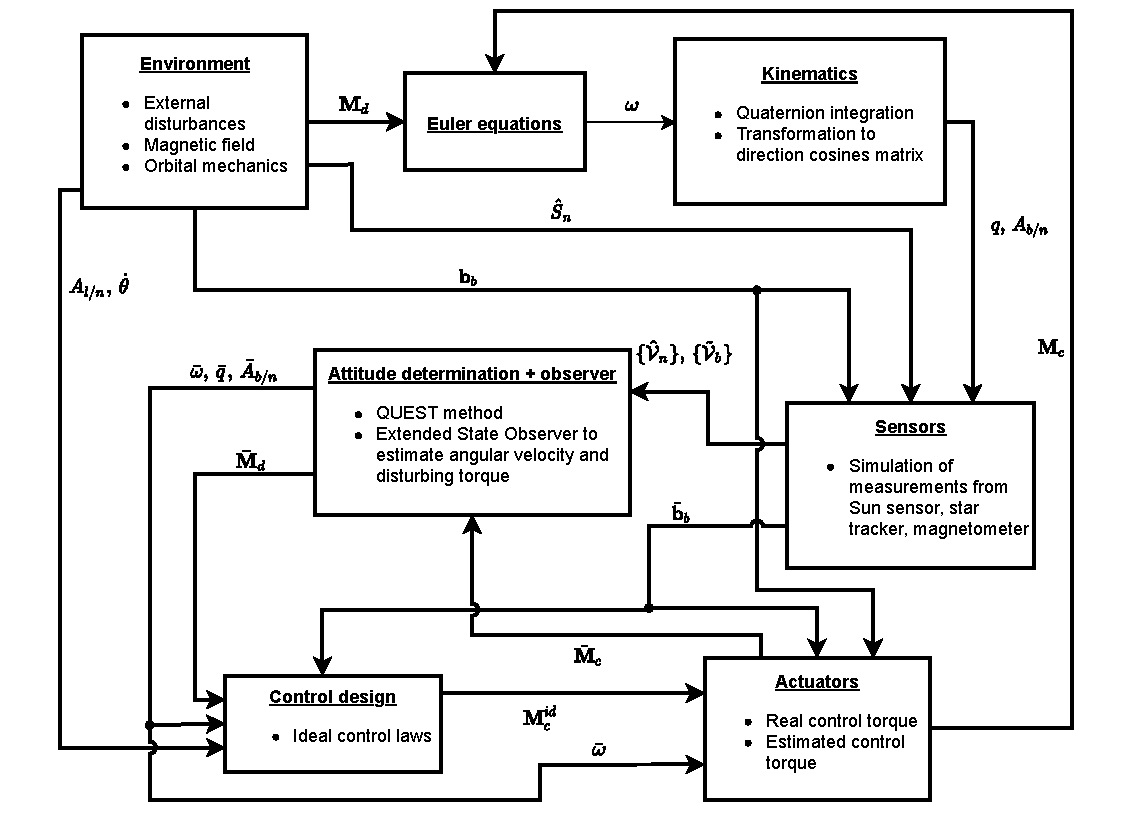
\includegraphics[width=\textwidth]{graphics/framework.pdf}
    \caption{Simulation framework}
    \label{fig:framework}
\end{figure}

\section{Results of the numerical simulation}

\subsection{Uncontrolled dynamics}

The uncontrolled dynamics of the satellite is simulated for one orbital period (equal to $\approx 1.54$ hours). The starting time is set to $t_0 = 0 \,s$. The initial conditions are the following:
\begin{equation*}
    \bm{\omega}_0 = \begin{bmatrix}
    20 & 14 & 3
    \end{bmatrix}^T \;
    ^{\circ}/s, \qquad
    q_0 = \begin{bmatrix}
    0 & 0 & 0 & 1
    \end{bmatrix}^T, \qquad
    \theta_0 = 0^{\circ}, \qquad
    \Bar{\mathbf{M}}_{d,0} = \begin{bmatrix}
    0 & 0 & 0
    \end{bmatrix}^T \; N \cdot m
\end{equation*}

The evolution in time of the disturbing torques, of the angular velocity and of the attitude quaternion are reported in \cref{fig:uncontrolled-disturbances,fig:uncontrolled-wq}.

\begin{figure}[h!]
    \centering
    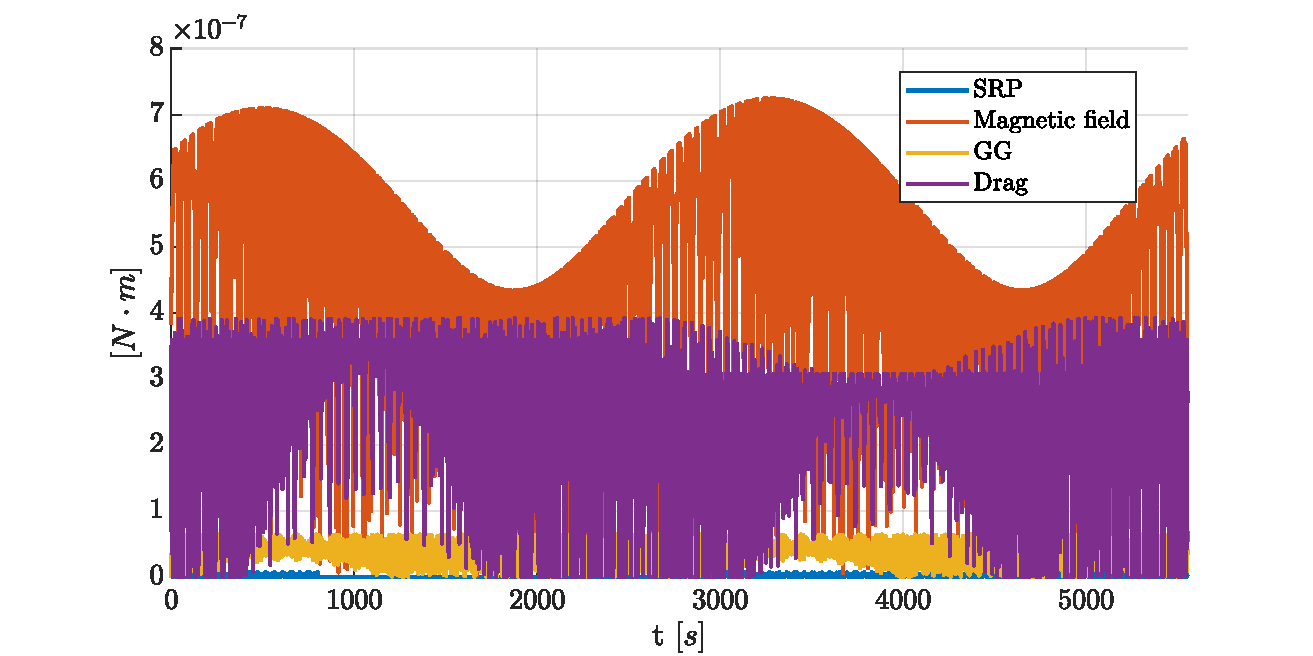
\includegraphics[width=0.8\textwidth]{graphics/uncontrolled/uncontrolled-disturbances.pdf}
    \caption{Evolution of the disturbances acting on the spacecraft}
    \label{fig:uncontrolled-disturbances}
\end{figure}

\begin{figure}[h!]
    \centering
    \subfloat[Angular velocity]{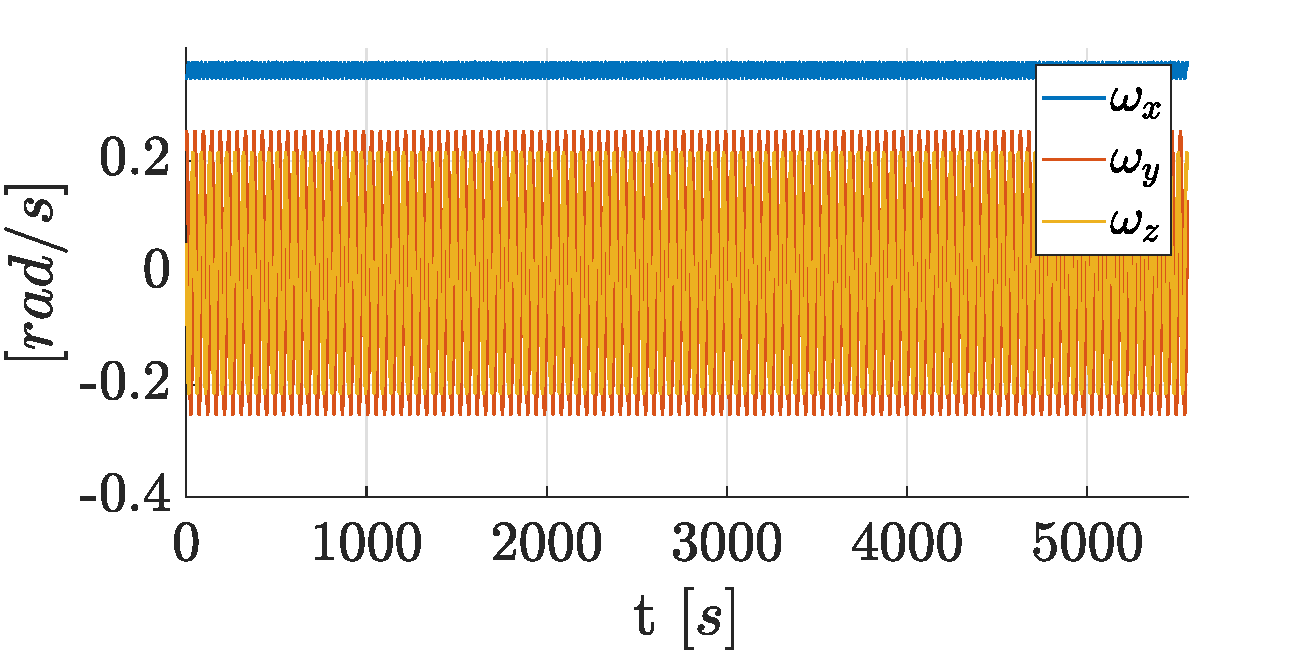
\includegraphics[width=0.49\textwidth]{graphics/uncontrolled/uncontrolled-w.pdf}}
    \subfloat[Quaternion]{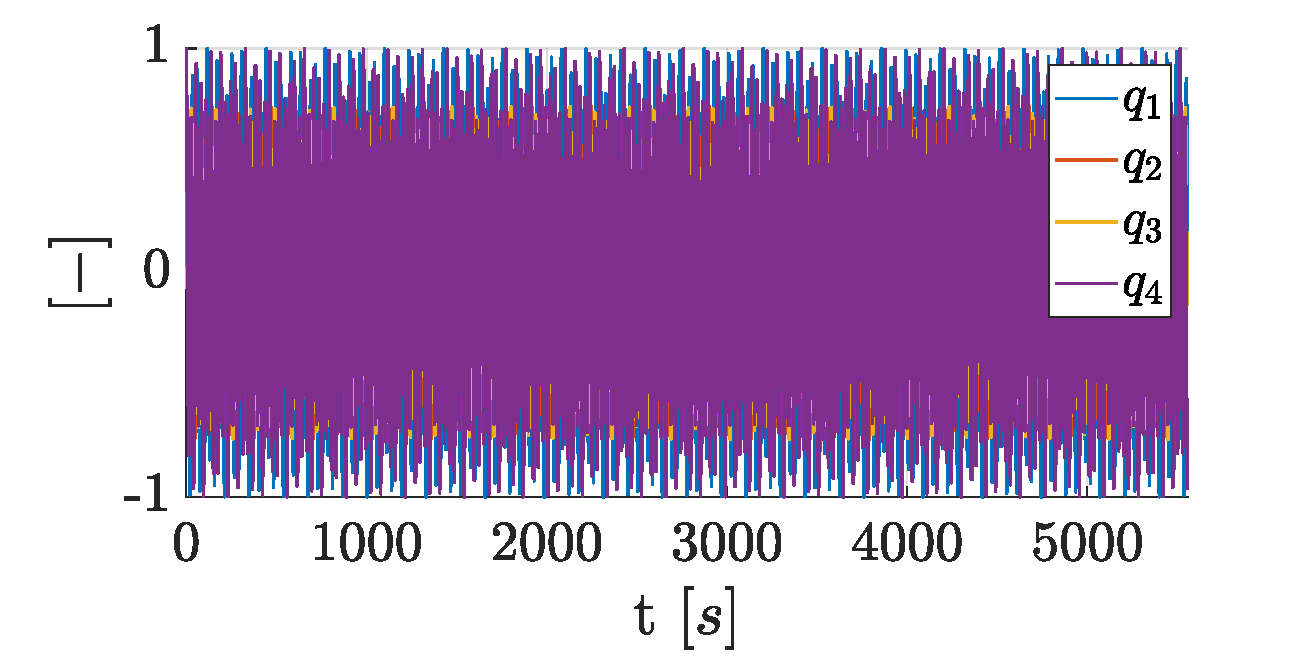
\includegraphics[width=0.49\textwidth]{graphics/uncontrolled/uncontrolled-q.pdf}}
    \caption{Evolution of $\bm{\omega}$ and $q$ in uncontrolled dynamics}
    \label{fig:uncontrolled-wq}
\end{figure}

\cref{tab:magnitude_torques} reports the maximum magnitude of the four disturbing torques. It is clear from the latter (as it also was from \cref{fig:uncontrolled-disturbances}) that the main disturbances are due to the magnetic field and the atmosphere, as the altitude of the orbit is relatively low. The impact that the gravity gradient and SRP have on the rotational dynamics is smaller.


\begin{table}[h!]
    \centering
    \caption{Maximum magnitude of the disturbing torques}
    \begin{tabular}{ccccc}
    \toprule
    \toprule
    & $\mathbf{M}_{\mathbf{b}}$ & $\mathbf{M}_{GG}$ & $\mathbf{M}_{drag}$ & $\mathbf{M}_{SRP}$\\
    \midrule
    Max. magnitude [$N\cdot m$] & 7.24 $\cdot 10^{-7}$ & 6.47 $\cdot 10^{-8}$ & 3.92 $\cdot 10^{-7}$ & 7.55 $\cdot 10^{-9}$ \\
    \bottomrule
    \bottomrule
    \end{tabular}
    \label{tab:magnitude_torques}
\end{table}

\subsection{Detumbling} \label{sec:control-tracking}

The detumbling phase is simulated from $t_0 = T = 5555.32 \, s$ to $t_{end} = 22220.93 \, s$. The initial conditions for both control strategies are set equal to:

\begin{equation*}
    \bm{\omega}_0 = \begin{bmatrix}
    21.10 & 7.38 & 10.55
    \end{bmatrix}^T \;
    ^{\circ}/s, \qquad
    q_0 = \begin{bmatrix}
    -0.17 & -0.15 & -0.14 & -0.96
    \end{bmatrix}^T, \qquad
    \theta_0 = 0^{\circ}
\end{equation*}
\begin{equation*}
    \Bar{\mathbf{M}}_{d,0} = \begin{bmatrix}
    0.03 & 0.12 & 0.49
    \end{bmatrix}^T \cdot 10^{-4} \, N \cdot m, \qquad
    \mathbf{h}_{r,0} = \begin{bmatrix}
    0 & 0 & 0 & 0
    \end{bmatrix}^T \; kg \, m^2/s
\end{equation*}

The results of the evolution of the angular velocity and of the attitude quaternions for both controls are presented in \cref{fig:detumbling-w,fig:detumbling-q}.

\begin{figure}[h!]
    \centering
    \subfloat[Spin rate damping]{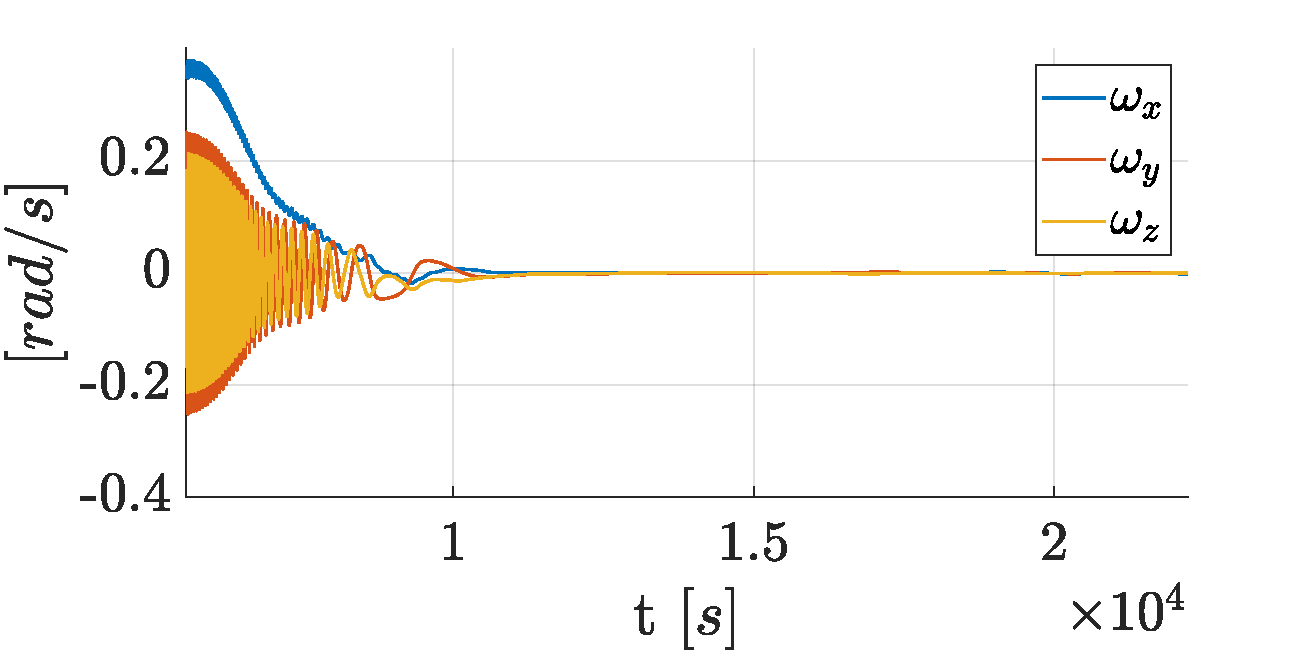
\includegraphics[width=0.49\textwidth]{graphics/detumbling-SRD/detumblingSRD-w.pdf}}
    \subfloat[Proportional control]{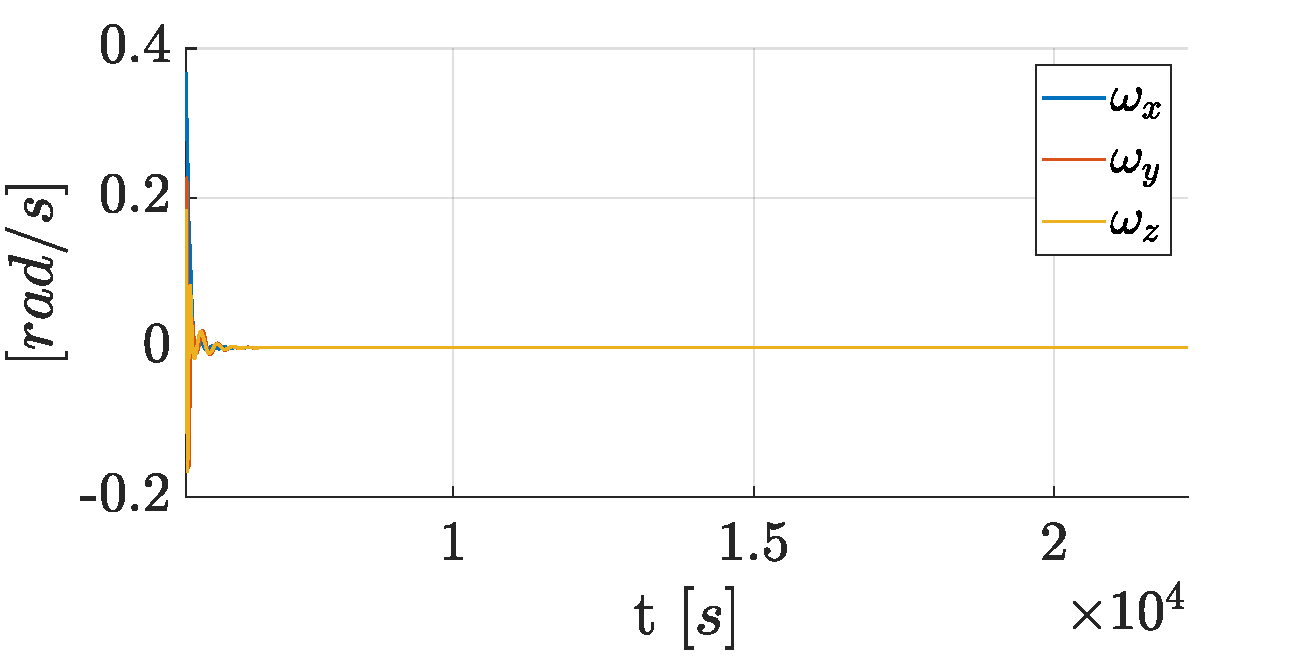
\includegraphics[width=0.49\textwidth]{graphics/detumbling-P/detumblingP-w.pdf}}
    \caption{Evolution of $\bm{\omega}$ in the detumbling phase}
    \label{fig:detumbling-w}
\end{figure}

\begin{figure}[h!]
    \centering
    \subfloat[Spin rate damping]{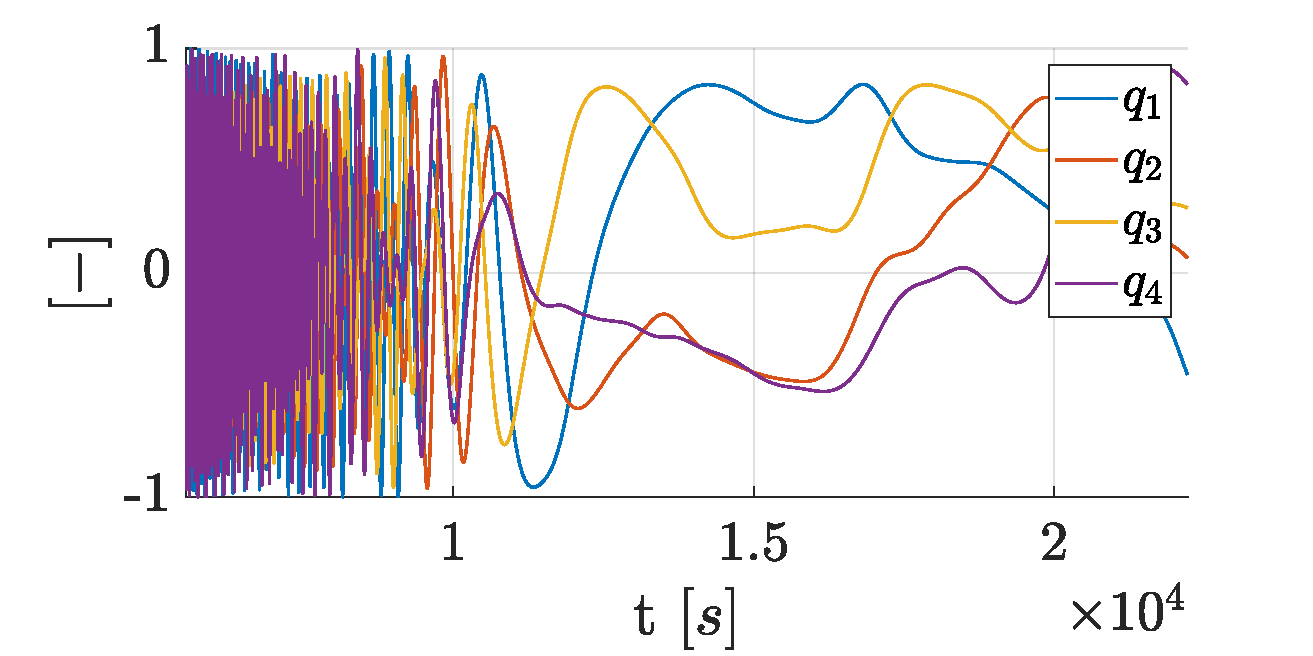
\includegraphics[width=0.49\textwidth]{graphics/detumbling-SRD/detumblingSRD-q.pdf}}
    \subfloat[Proportional control]{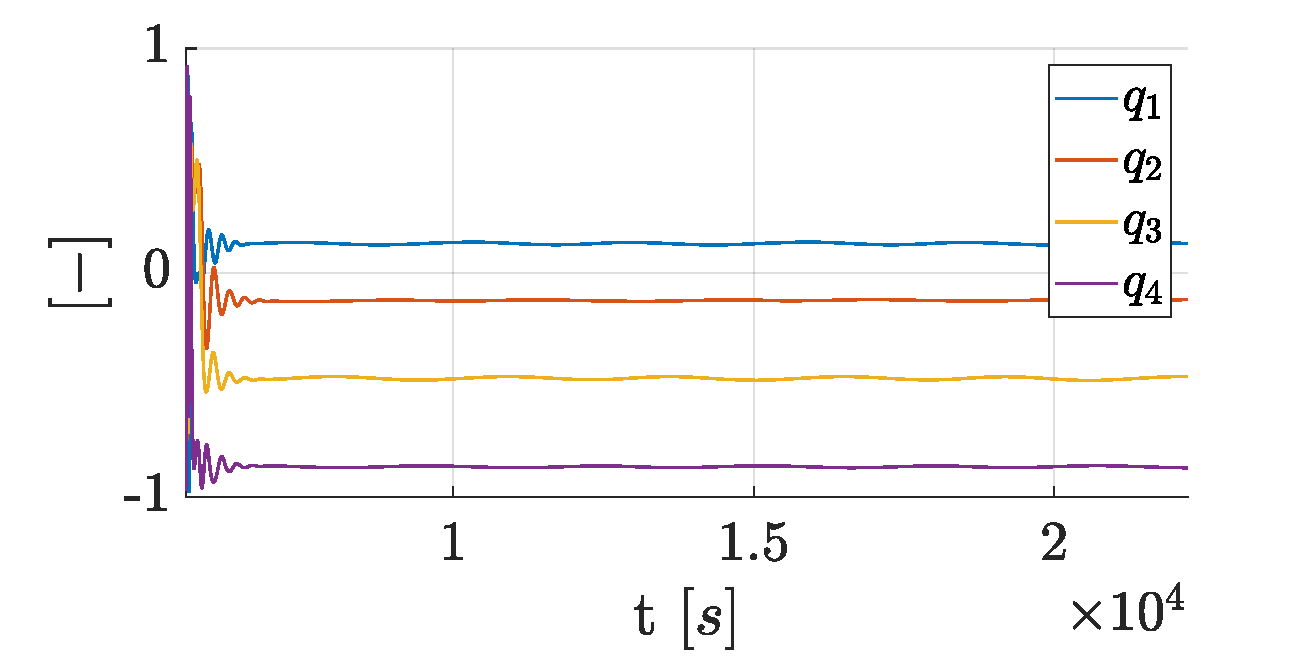
\includegraphics[width=0.49\textwidth]{graphics/detumbling-P/detumblingP-q.pdf}}
    \caption{Evolution of $q$ in the detumbling phase}
    \label{fig:detumbling-q}
\end{figure}

The proportional control proves to be more efficient: $\bm{\omega}$ quickly drops close to zero and the attitude quaternion stabilizes itself after $\approx 1000 \, s$. In the spin rate damping, the detumbling can be considered to be completed in $\approx 5500 \, s \approx 1\, T$. All the components of the angular velocity face a slower decay compared to the other strategy: this is due to the inherent nature of the magnetorquer, which is less powerful than the RWs and can rarely generate the required control torque, as explained in \cref{sec:control}. The values of the angular velocity at the end of the control phase are reported in \cref{tab:detumbling_finalW}. It is clear again that the proportional control guarantees better performances.

\begin{table}[h!]
    \centering
    \caption{Values of the angular velocity after the detumbling phase}
    \begin{tabular}{cc}
    \toprule
    \toprule
    \multicolumn{2}{c}{\textbf{$\bm{\omega}$ after the detumbling control} $[rad/s]$} \\
    \midrule
    Spin rate damping & Proportional control \\
    \midrule
    $\begin{bmatrix} -16.21 & 0.01 & -0.03 \end{bmatrix}^T \cdot 10^{-2}$  &  $\begin{bmatrix} 0.15 & -0.21 & 0.09 \end{bmatrix}^T \cdot 10^{-4}$ \\
    \bottomrule
    \bottomrule
    \end{tabular}
    \label{tab:detumbling_finalW}
\end{table}

The performances of the QUEST estimator and of the ESO are presented through the plots in \cref{fig:detumbling-estQ,fig:detumbling-estW}. In both strategies, the estimation of both $q$ and $\bm{\omega}$ is not satisfactory in the first time instants. The error on the attitude quaternion goes below $10^{-4}$ in $\approx 200 \,s$ for the proportional control, while for the SRD the same value is reached only after $\approx 2700 \,s$. The fact that the decay rate of the error is different for the two strategies could be attributed to the higher frequency of oscillation of $\bm{\omega}$ in the first part of the SRD compared the proportional control. The time variations of the quaternion are very fast, so the sensors for the attitude determination (especially the star tracker, whose update rate is slow) might not keep up at generating updated measurements, degrading the performances of the QUEST algorithm. The same phenomenon can be noticed in the estimation of the angular velocity: for the proportional control, the error drops close to $10^{-3}\, rad/s$ after $1000\, s$, while in the SRD it takes $\approx 2700 \,s$. The decay of the error on the angular velocity is slower with respect to the estimation of $q$ as $\bm{\omega}$ goes through multiple steps in its determination (low-pass filtering of $\Bar{q}$ $\rightarrow$ numerical derivation of $\Bar{q}$ $\rightarrow$ ESO), while the quaternion is a direct product of the QUEST algorithm.

\begin{figure}[h!]
    \centering
    \subfloat[Spin rate damping]{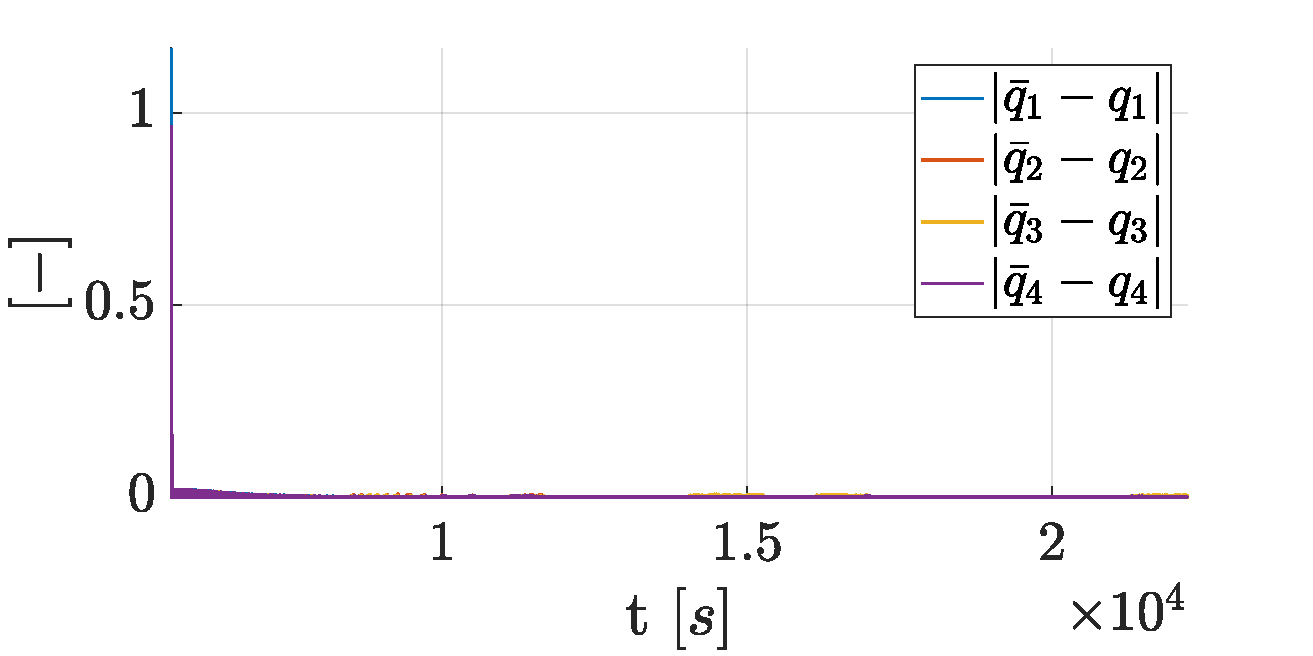
\includegraphics[width=0.49\textwidth]{graphics/detumbling-SRD/detumblingSRD-estQ.pdf}}
    \subfloat[Proportional control]{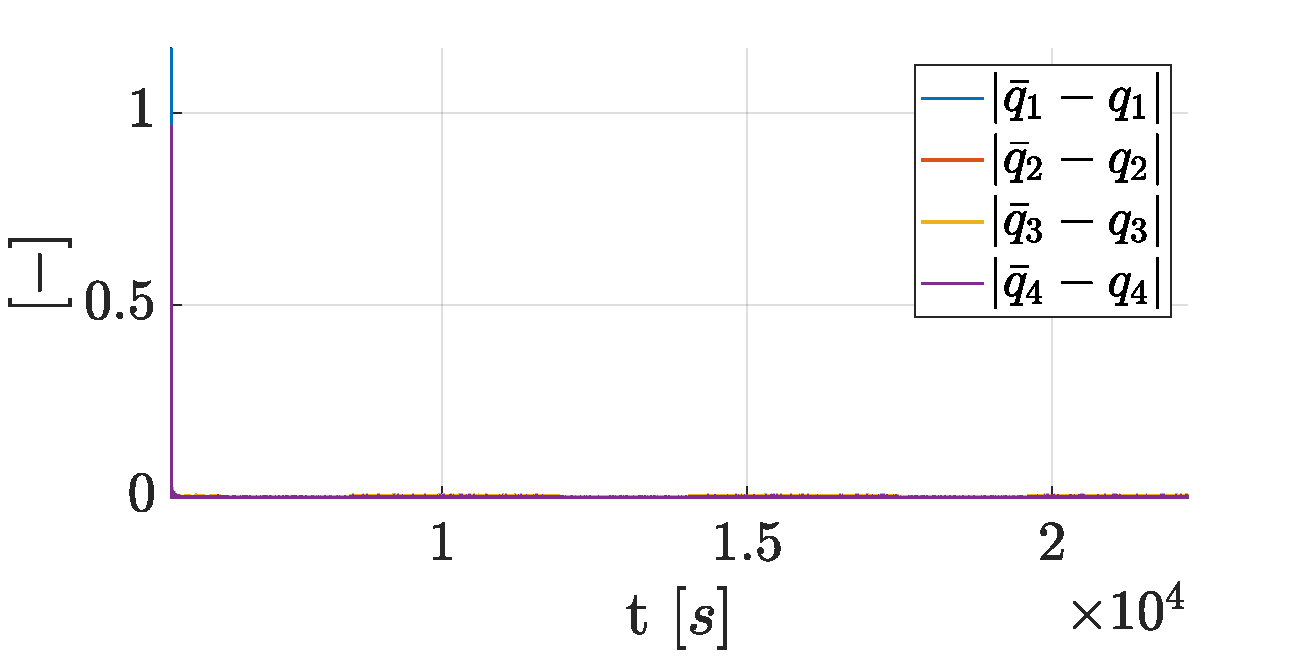
\includegraphics[width=0.49\textwidth]{graphics/detumbling-P/detumblingP-estQ.pdf}}
    \caption{Evolution of the estimation error on $q$ in the detumbling phase}
    \label{fig:detumbling-estQ}
\end{figure}

\begin{figure}[h!]
    \centering
    \subfloat[Spin rate damping]{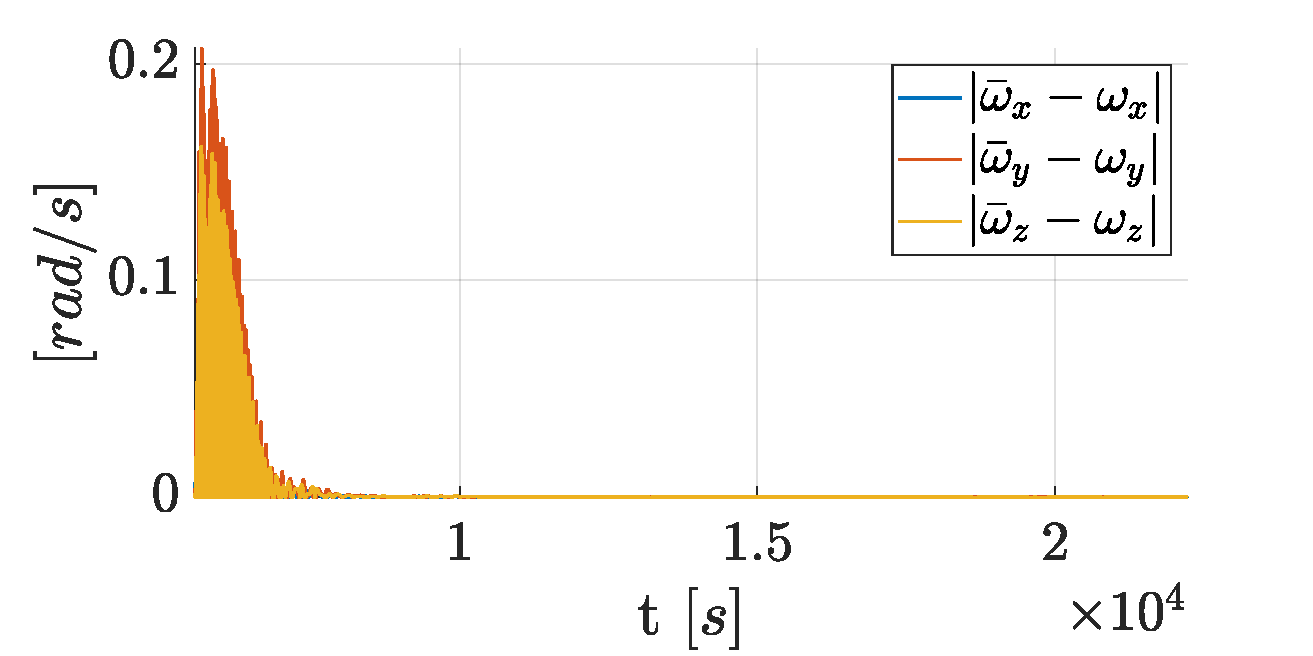
\includegraphics[width=0.49\textwidth]{graphics/detumbling-SRD/detumblingSRD-estW.pdf}}
    \subfloat[Proportional control]{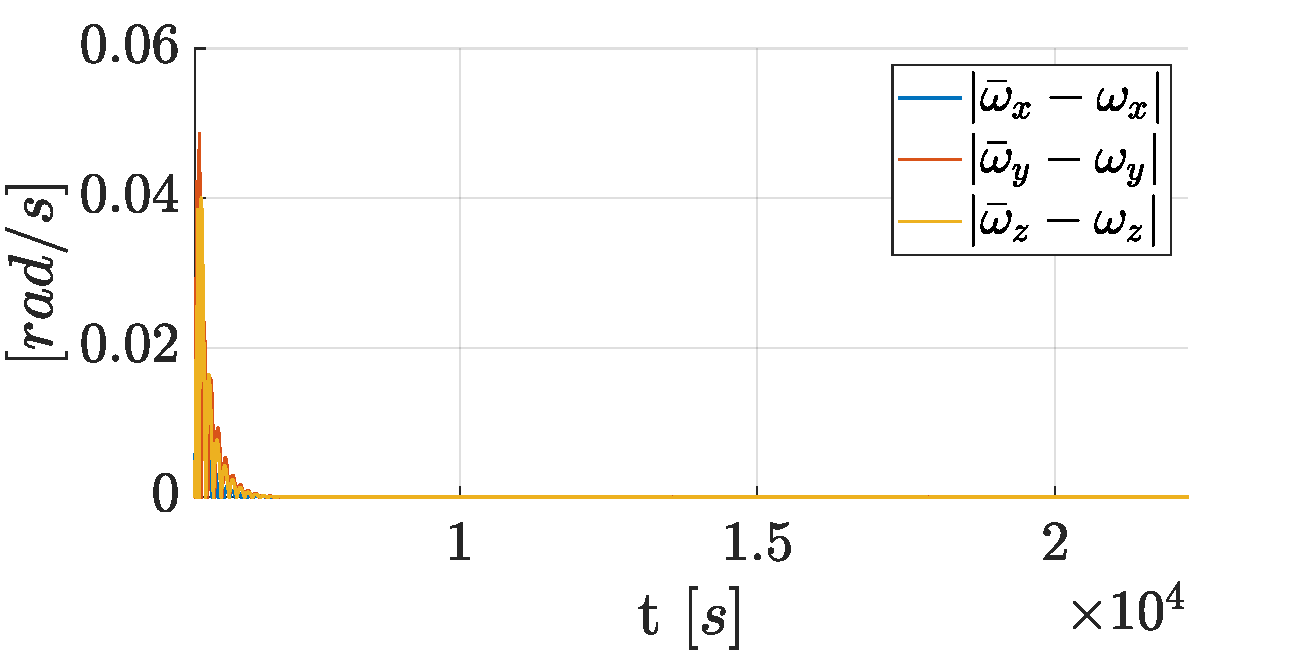
\includegraphics[width=0.49\textwidth]{graphics/detumbling-P/detumblingP-estW.pdf}}
    \caption{Evolution of the estimation error on $\bm{\omega}$ in the detumbling phase}
    \label{fig:detumbling-estW}
\end{figure}

\cref{fig:detumblingSRD-D} reports the values of the components of the magnetic dipole which the magnetorquer must generate in the spin rate damping. The actuator gets saturated in all the three directions in the first part of the control.

\begin{figure}[h!]
    \centering
    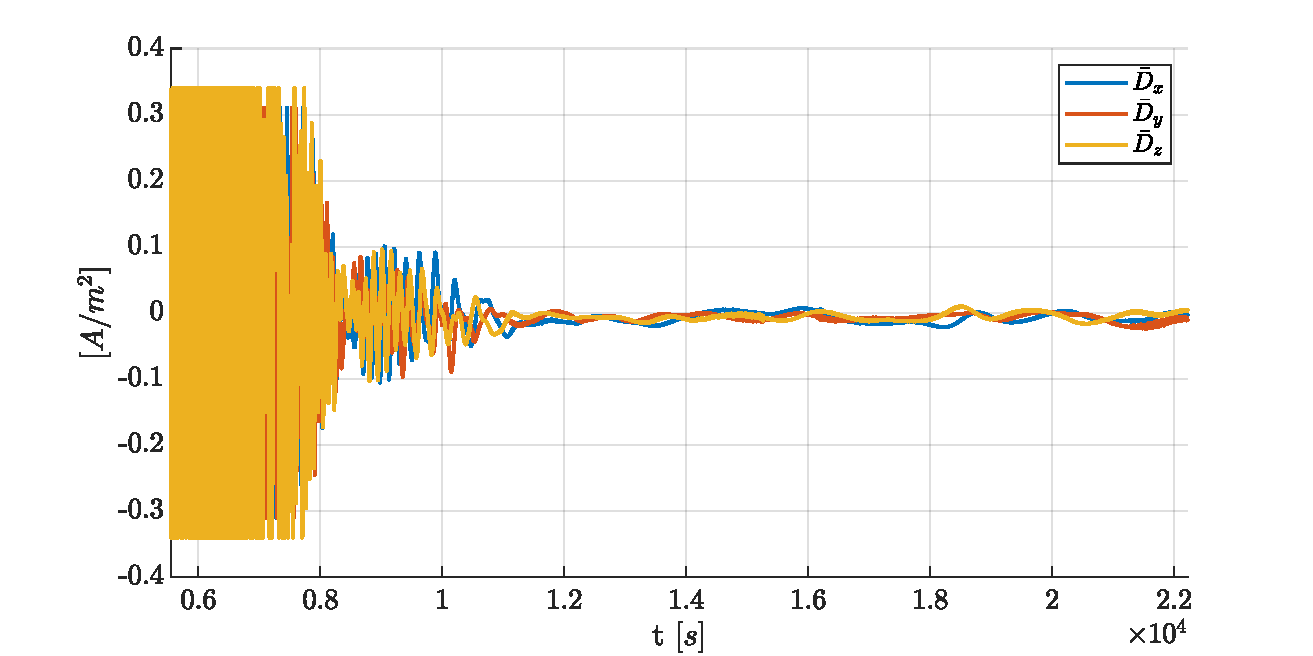
\includegraphics[width=0.8\textwidth]{graphics/detumbling-SRD/detumblingSRD-D.pdf}
    \caption{Evolution of the magnetic dipole of the magnetorquer}
    \label{fig:detumblingSRD-D}
\end{figure}

\subsection{Tracking}

The tracking phase is simulated from $t_0 = 22220.93 \, s$ to $t_{end} = 38886.63 \, s$. The initial conditions for this simulation are retrieved from the final conditions of the detumbling phase with the proportional control.

\begin{equation*}
    \bm{\omega}_0 = \begin{bmatrix}
    0.15 & -0.21 & 0.09
    \end{bmatrix}^T \cdot 10^{-4} \;
    rad/s, \qquad
    q_0 = \begin{bmatrix}
    0.13 & -0.11 & -0.46 & -0.86
    \end{bmatrix}^T, \qquad
    \theta_0 = 0^{\circ}
\end{equation*}
\begin{equation*}
    \Bar{\mathbf{M}}_{d,0} = \begin{bmatrix}
    -0.08 & -0.05 & -0.46
    \end{bmatrix}^T \cdot 10^{-6} \, N \cdot m, \qquad
    \mathbf{h}_{r,0} = \begin{bmatrix}
    -1.14 & 16.52 & 13.6 & -4.06
    \end{bmatrix}^T \; mN \cdot ms
\end{equation*}

The results of the simulations are presented in the plots below. It is clear from \cref{fig:tracking-w} and \cref{fig:tracking-Abn_pe} that the control logic fulfils the requirements. The first two components of the angular velocity quickly drop to zero, while the third one tracks the angular speed of the LVLH frame $\Dot{\theta}$: as it is possible to see in \cref{fig:tracking-w_zoom}, $\omega_z$ oscillates around the orbital mean motion $n = 1/T$. The evolution of direction cosines becomes periodic. The pointing error decays rapidly, reaching values close to $10^{-3}\,{}^{\circ}$ in approximately $1300 \, s$, thus satisfying the mission requirements.

\begin{figure}[h!]
    \centering
    \subfloat[Angular velocity]{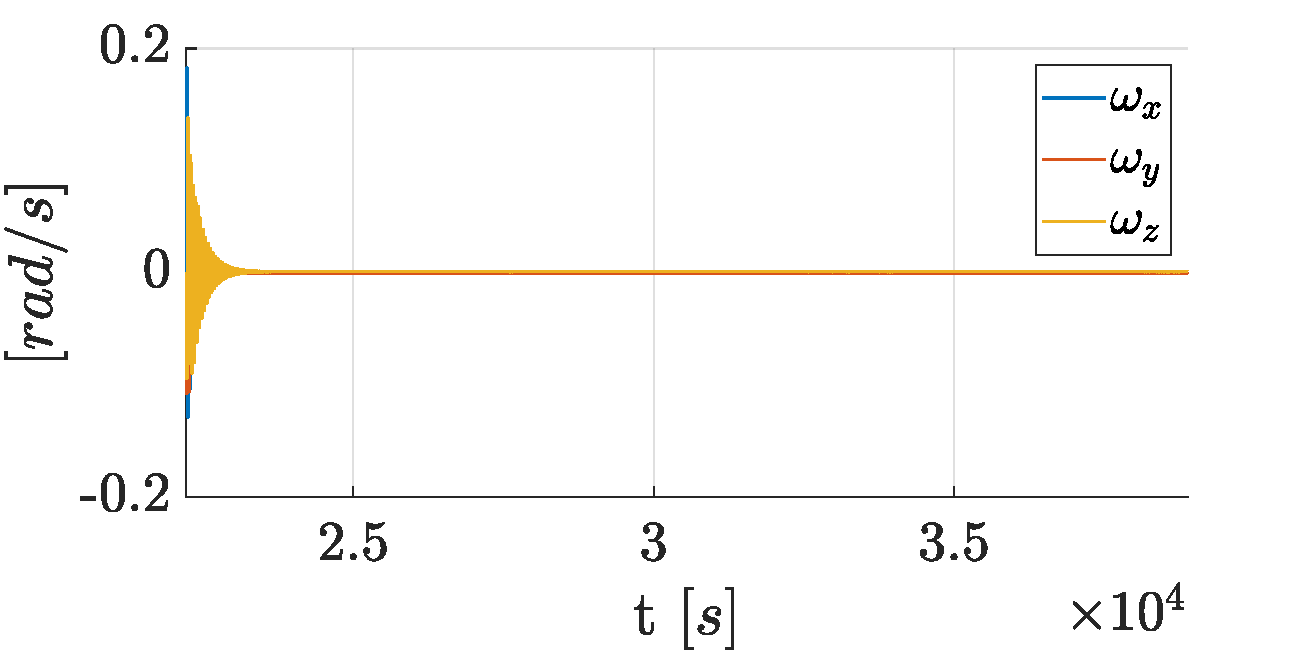
\includegraphics[width=0.49\textwidth]{graphics/tracking/tracking-w.pdf}}
    \subfloat[Angular velocity (detail) \label{fig:tracking-w_zoom}]{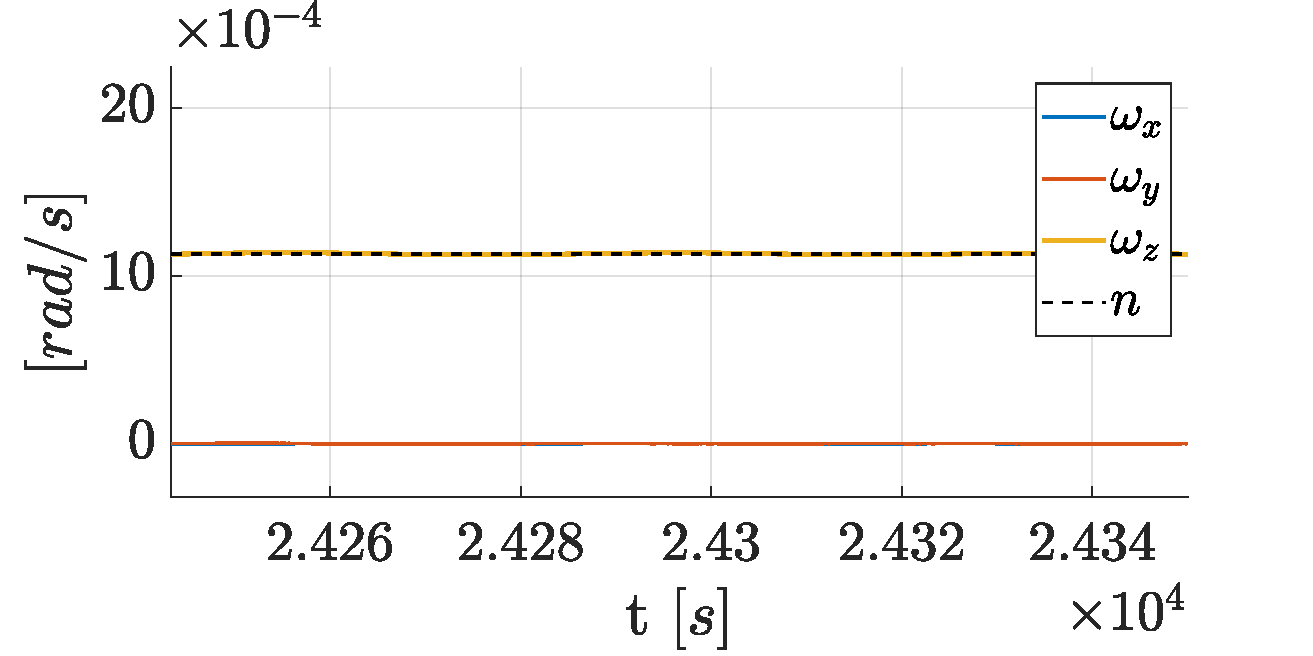
\includegraphics[width=0.49\textwidth]{graphics/tracking/tracking-w_zoom.pdf}}
    \caption{Evolution of $\bm{\omega}$ in the tracking phase}
    \label{fig:tracking-w}
\end{figure}

\begin{figure}[h!]
    \centering
    \subfloat[Direction cosines matrix]{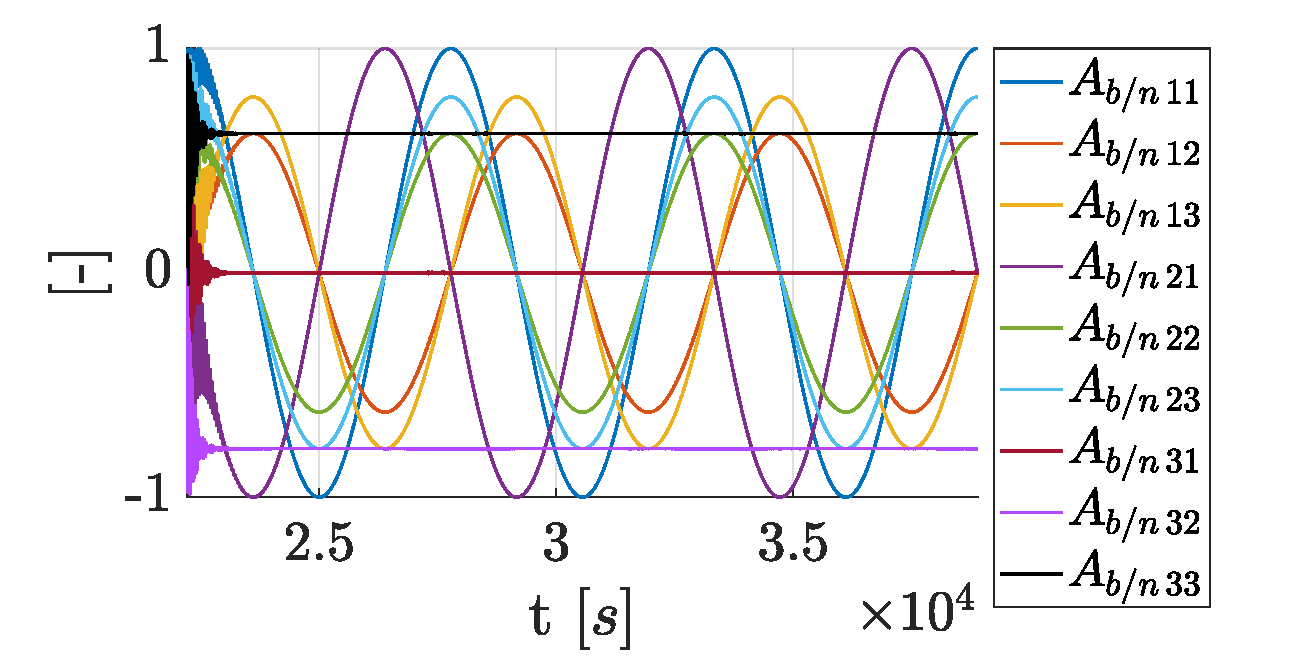
\includegraphics[width=0.49\textwidth]{graphics/tracking/tracking-Abn.pdf}}
    \subfloat[Pointing error]{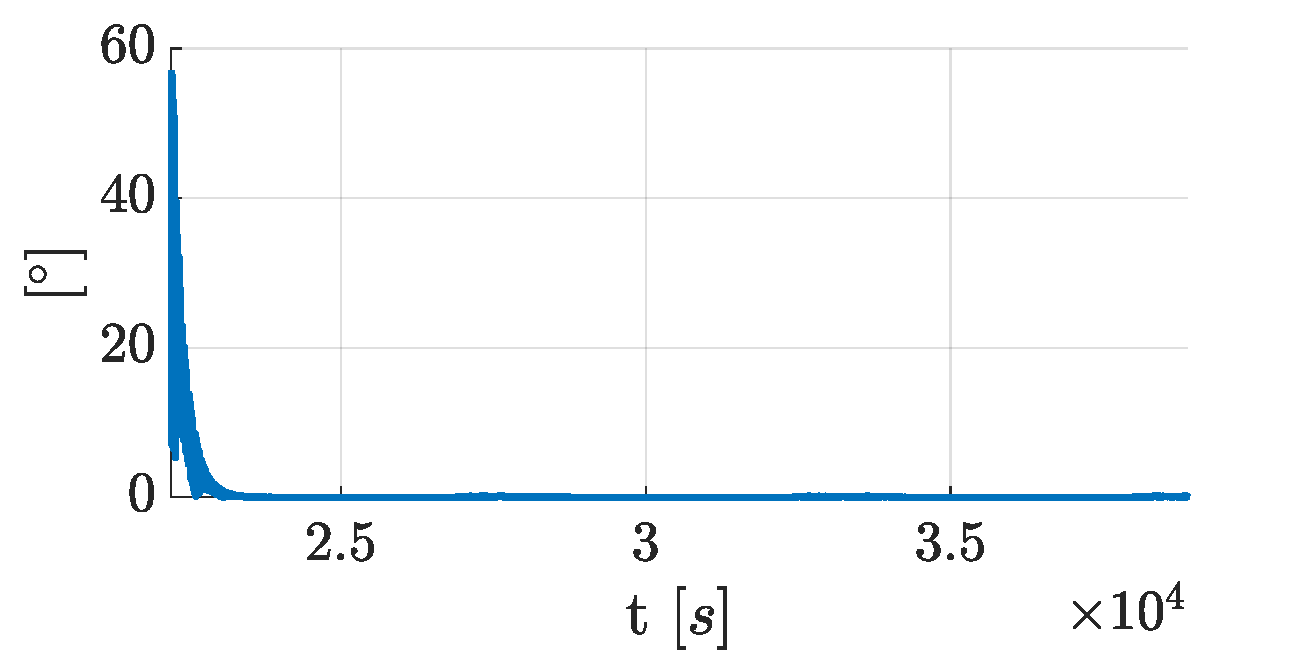
\includegraphics[width=0.49\textwidth]{graphics/tracking/tracking-pe.pdf}}
    \caption{Evolution of $A_{b/n}$ and of the pointing error in the tracking phase}
    \label{fig:tracking-Abn_pe}
\end{figure}

For this phase, the performance of the estimators (QUEST + ESO) are presented through the plots in \cref{fig:tracking-estWabn}. The errors associated to the direction cosines matrix (\cref{fig:tracking-estAbn}), which is derived directly from the QUEST method via \cref{eq:dcm}, rapidly drop to zero. The estimation of the angular velocity becomes satisfactory only after $\approx 1200 \, s$ (with $\| \bar{\bm{\omega}} - \bm{\omega} \|$ in the order of $10^{-5} \, rad/s$). The reasons of this behaviour are the same as the ones explained in \cref{sec:control-tracking}. The same trend can be observed also in the estimations of the disturbing and control torques (\cref{fig:tracking-estMd,fig:tracking-estMc}), as they come from the dynamics of the ESO which involves $\bar{\bm{\omega}}$. 

\begin{figure}[h!]
    \centering
    \subfloat[Direction cosine matrix \label{fig:tracking-estAbn}]{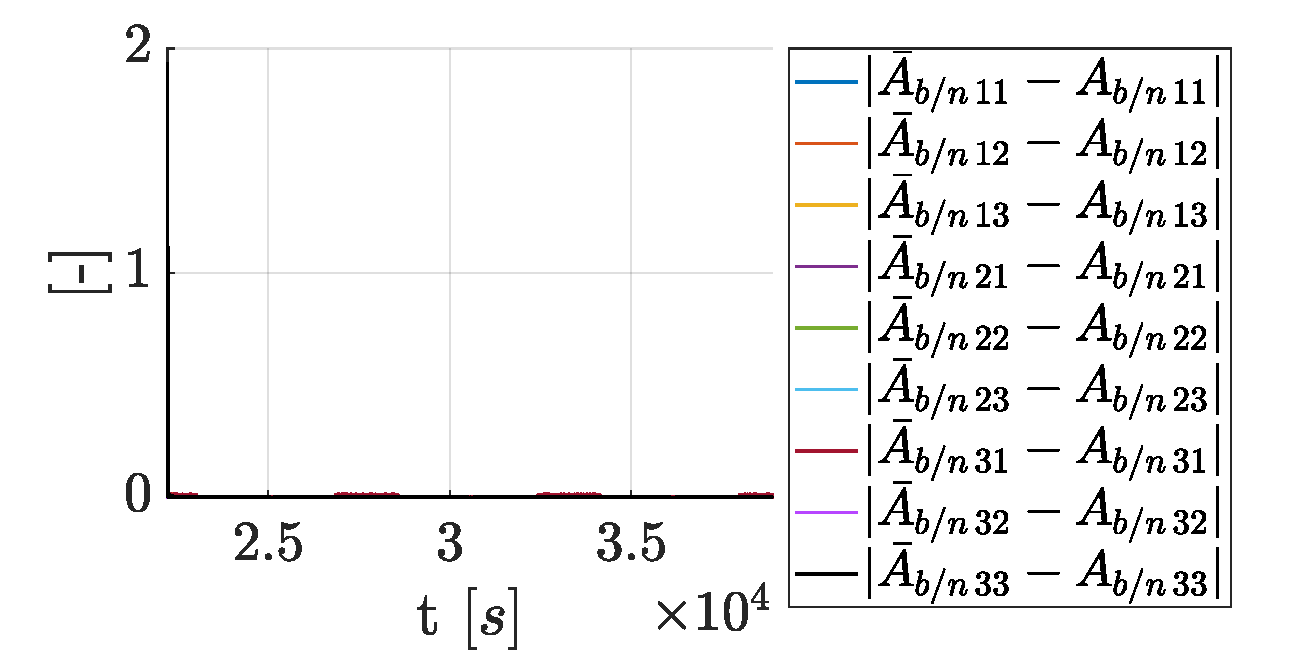
\includegraphics[width=0.49\textwidth]{graphics/tracking/tracking-estAbn.pdf}}
    \subfloat[Angular velocity]{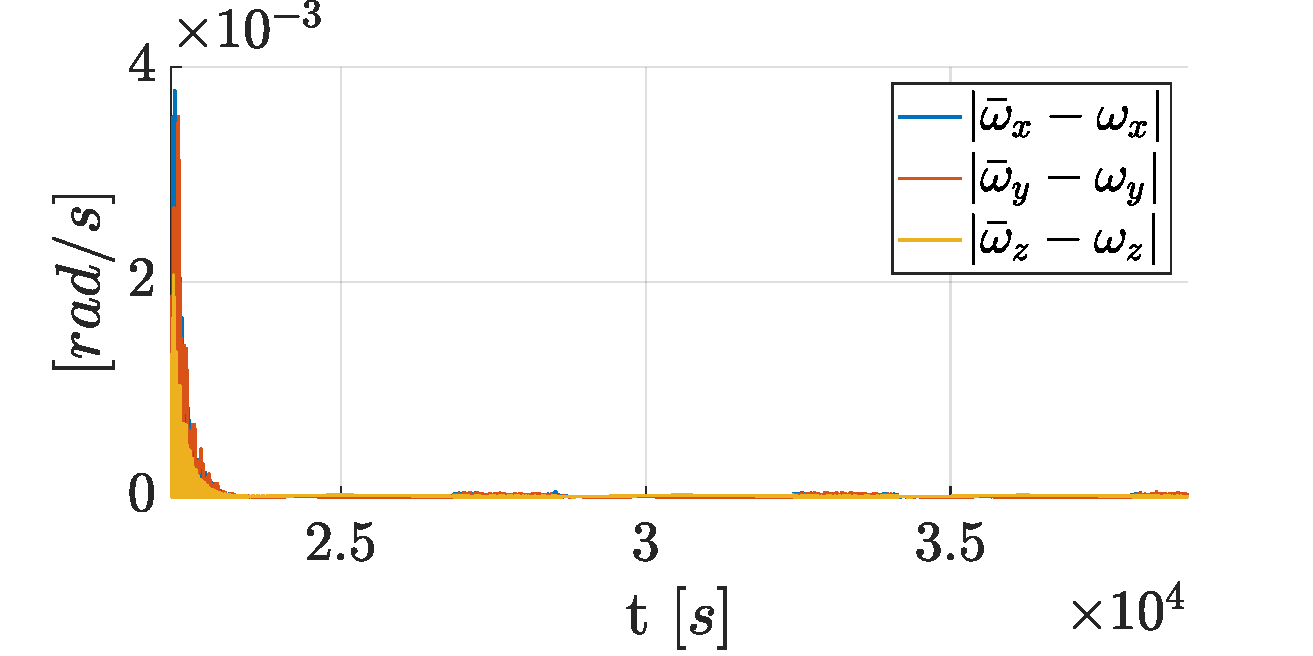
\includegraphics[width=0.49\textwidth]{graphics/tracking/tracking-estW.pdf}}
    \caption{Evolution of the estimation errors ($A_{b/n}$ and $\bm{\omega}$) in the tracking phase}
    \label{fig:tracking-estWabn}
\end{figure}   

\begin{figure}[h!]
    \subfloat[Disturbing torque \label{fig:tracking-estMd}]{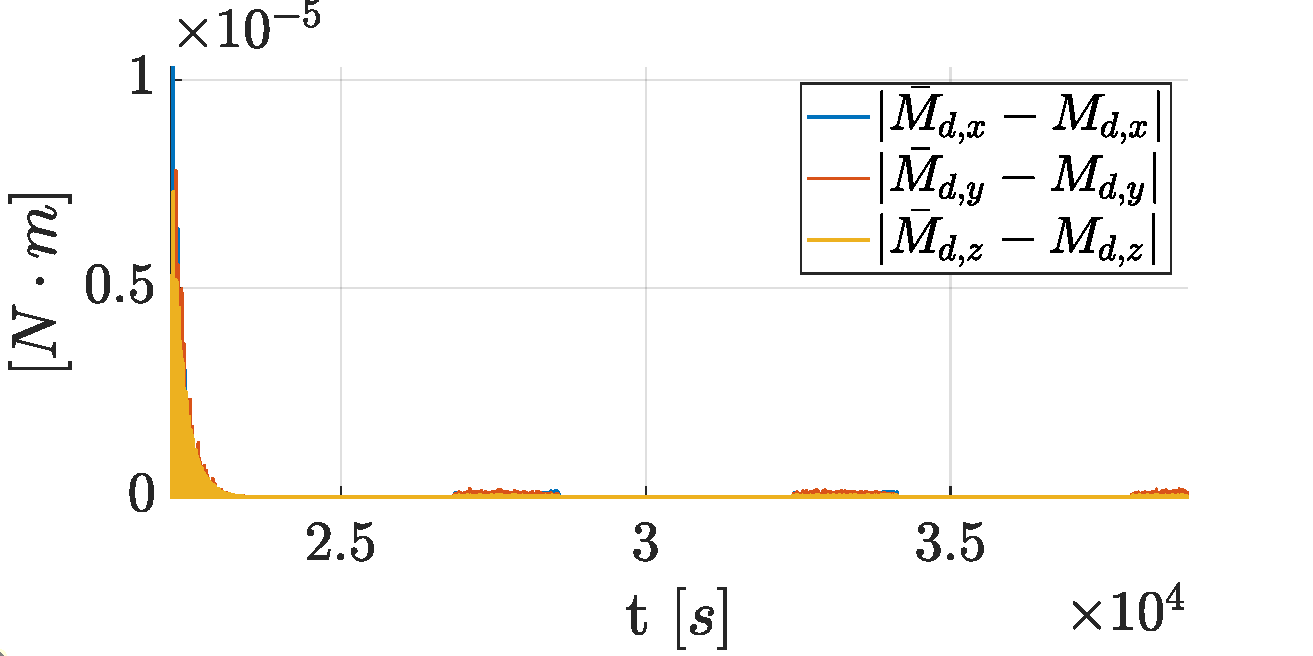
\includegraphics[width=0.49\textwidth]{graphics/tracking/tracking-estMd.pdf}}
    \subfloat[Control torque \label{fig:tracking-estMc}]{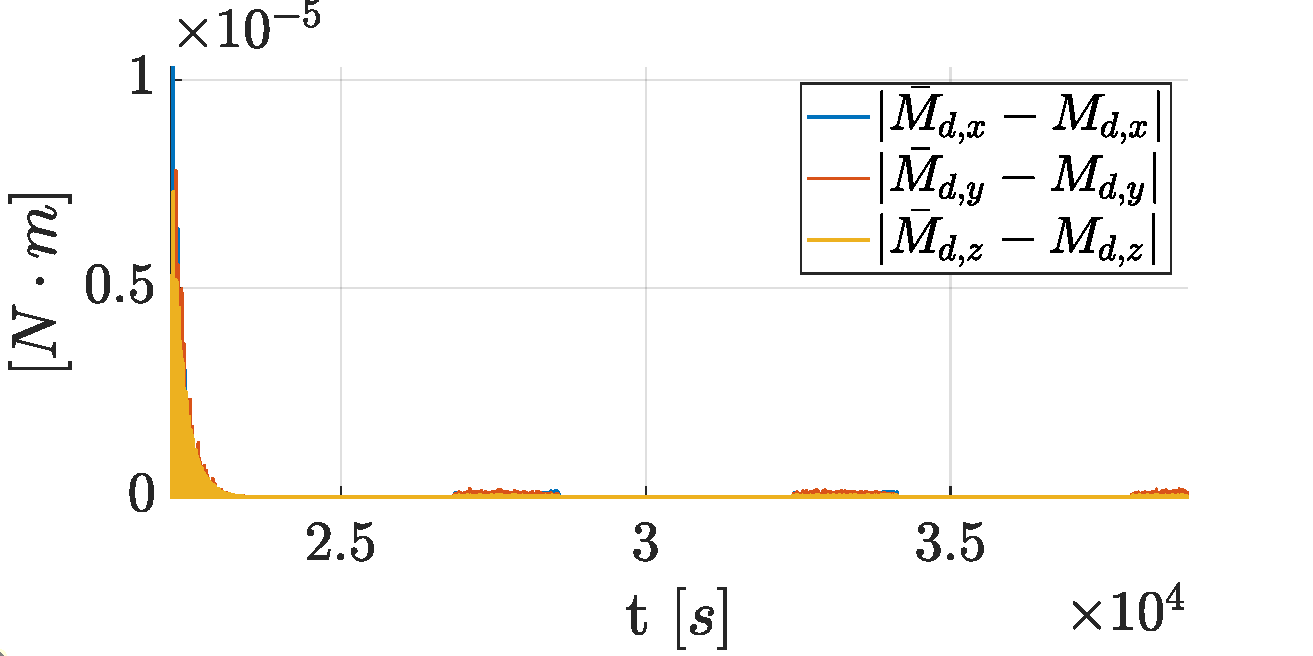
\includegraphics[width=0.49\textwidth]{graphics/tracking/tracking-estMd.pdf}}
    \caption{Evolution of the estimation errors ($\mathbf{M}_d$ and $\mathbf{M}_c$) in the tracking phase}
    \label{fig:tracking-estM}
\end{figure}

The maximum estimation errors on the torques (for $t > \bar{t} = 30482.89 \, s$) are presented in \cref{tab:torques_estimation}. The search region for the maxima is reduced in order to exclude the first time instants, in which the dynamics of the estimation is not settled yet. The error on the disturbing torque is approximately in the order of the torques itself (\cref{tab:magnitude_torques}). Nevertheless, it is possible to notice that this uncertainty is filtered out when estimating the control torque (whose error is extremely low), so it does not affect the robustness of the control system.

\begin{table}[h!]
    \centering
    \caption{Maximum estimation errors on the disturbing and control torques}
    \begin{tabular}{cc}
    \toprule
    \toprule
    $\max_{t > \bar{t}} \; \| \bar{\mathbf{M}}_d - \mathbf{M}_d \|$ & $\max_{t > \bar{t}} \; \| \bar{\mathbf{M}}_c - \mathbf{M}_c \|$ \\
    \midrule
    $2.02 \cdot 10^{-7} \, N \cdot m$ & $2.12 \cdot 10^{-20} \, N \cdot m$ \\
    \bottomrule
    \bottomrule
    \end{tabular}
    \label{tab:torques_estimation}
\end{table}

The angular momentum of the reaction wheels, whose evolution is reported in \cref{fig:tracking-hr}, oscillates periodically with monotonous increments of the DC offsets. The actuator will eventually reach saturation, hence a de-saturation mechanism shall be developed. On the other hand, the torque provided to the wheels $\mathbf{M}_r$ (\cref{fig:tracking-mr}) show a fast decay as the spacecraft reaches the desired attitude, after a first peak phase.

\begin{figure}[h!]
    \centering
    \subfloat[Angular momentum \label{fig:tracking-hr}]{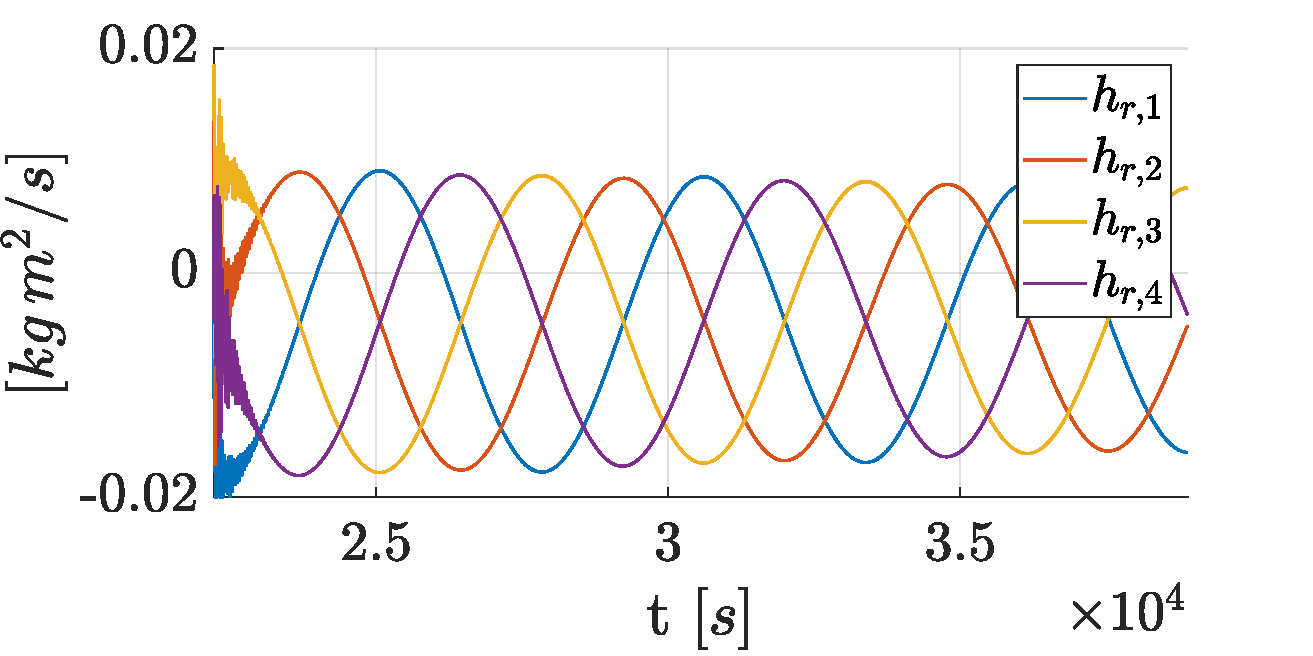
\includegraphics[width=0.49\textwidth]{graphics/tracking/tracking-hr.pdf}}
    \subfloat[Torque provided to the wheels \label{fig:tracking-mr}]{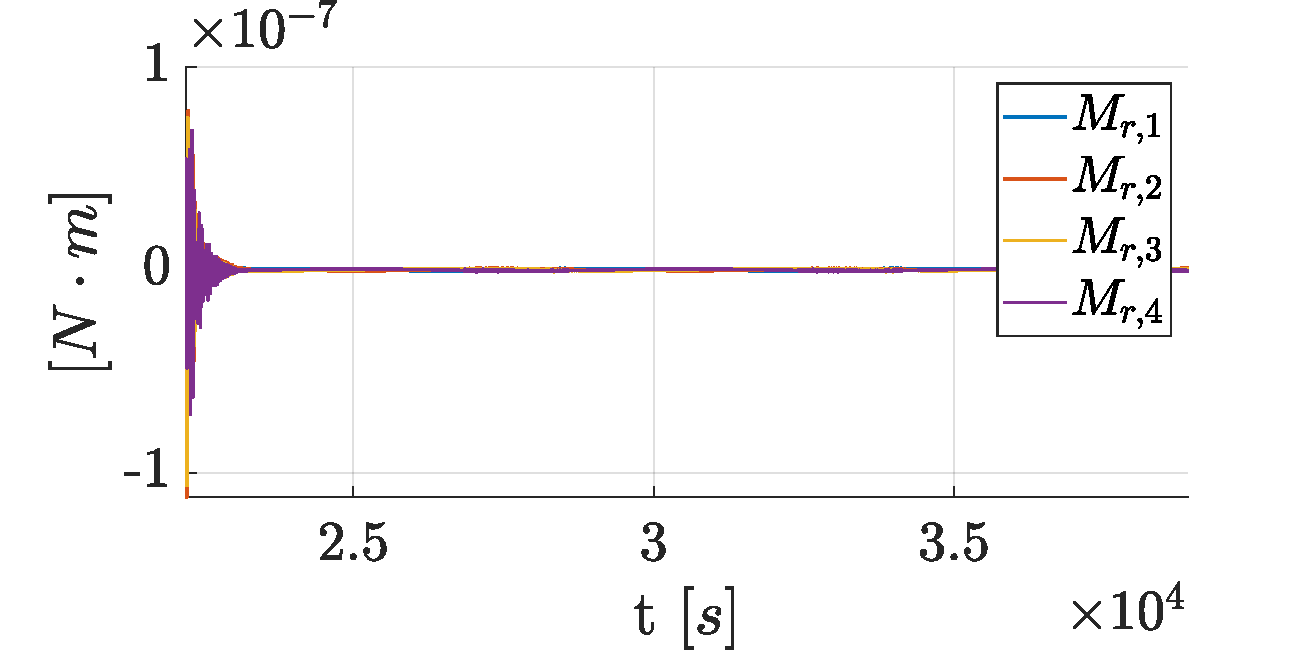
\includegraphics[width=0.49\textwidth]{graphics/tracking/tracking-Mr.pdf}}
    \caption{Evolution of $\mathbf{h}_r$ and $\mathbf{M}_r$ in the tracking phase}
    \label{fig:tracking-rw}
\end{figure}

\section{Simulation of off-nominal conditions}

The roubstness of the designed control design is verified by simulating three cases of off-nominal conditions. The parameters which vary are the inertia matrix, the residual magnetic dipole of the spacecraft and the initial conditions for the angular velocity and attitude quaternion. These simulated properties are reported in \cref{tab:off-nominal}.

\begin{table}[h!]
    \centering
    \caption{Properties for simulation of off-nominal conditions}
    \begin{tabular}{cccc}
    \toprule
    \toprule
    & \textbf{Case 1} & \textbf{Case 2} & \textbf{Case 3} \\
    \midrule
    $I \; [kg \cdot dm^2]$ & $\begin{bmatrix} 6.01 & -0.78 & 0.90 \\
    -0.78 & 7.71 & 0.05 \\
    0.90 & 0.05 & 9.81
    \end{bmatrix}$ & $\begin{bmatrix} 5.04 & 1.00 & -0.60 \\
    1.00 & 6.50 & 0.40 \\
    -0.60 & 0.40 & 8.41
    \end{bmatrix}$ & $\begin{bmatrix} 4.60 & -0.50 & -1.20 \\
    -0.50 & 8.31 & 1.10 \\
    -1.20 & 1.10 & 5.7
    \end{bmatrix}$\\
    \midrule
    $\mathbf{D}_r \; [A/m^2]$ & $ \begin{bmatrix} 0.02 & 0.04 & -0.10
    \end{bmatrix}$ & $ \begin{bmatrix} -0.04 & 0.05 & 0.10
    \end{bmatrix}$ & $ \begin{bmatrix} 0.08 & -0.05 & 0.04
    \end{bmatrix}$ \\
    \midrule
    $\bm{\omega}_0 \; [{}^{\circ}/s]$ & $\begin{bmatrix} 1 & 2 & 5
    \end{bmatrix}$ & $\begin{bmatrix} 4 & 10 & 9
    \end{bmatrix}$ & $\begin{bmatrix} 7 & 2 & 6
    \end{bmatrix}$\\
    \midrule
    $q_0 \; [-]$ & $\begin{bmatrix} 0.32 & 0.64 & 0.13 & 0.68
    \end{bmatrix}$ & $\begin{bmatrix} 0.55 & 0.30 & 0.75 & 0.19
    \end{bmatrix}$ & $\begin{bmatrix} 0.71 & 0.11 & 0.31 & 0.62
    \end{bmatrix}$ \\
    \bottomrule
    \bottomrule
    \end{tabular}
    \label{tab:off-nominal}
\end{table}

The cases are simulated only in the detumbling phase (with the proportional control) and in the tracking phase. The starting time of the simulations is set to $t = 0 \, s$ and each control phase lasts three orbital periods (as in the nominal case). The results of the analysis is reported through two of the most significant parameters ($\| \bm{\omega} \|$ for the detumbling phase and the pointing error in the tracking phase) in \cref{fig:offNominal-w,fig:offNominal-pe}.

\begin{figure}[h!]
    \centering
    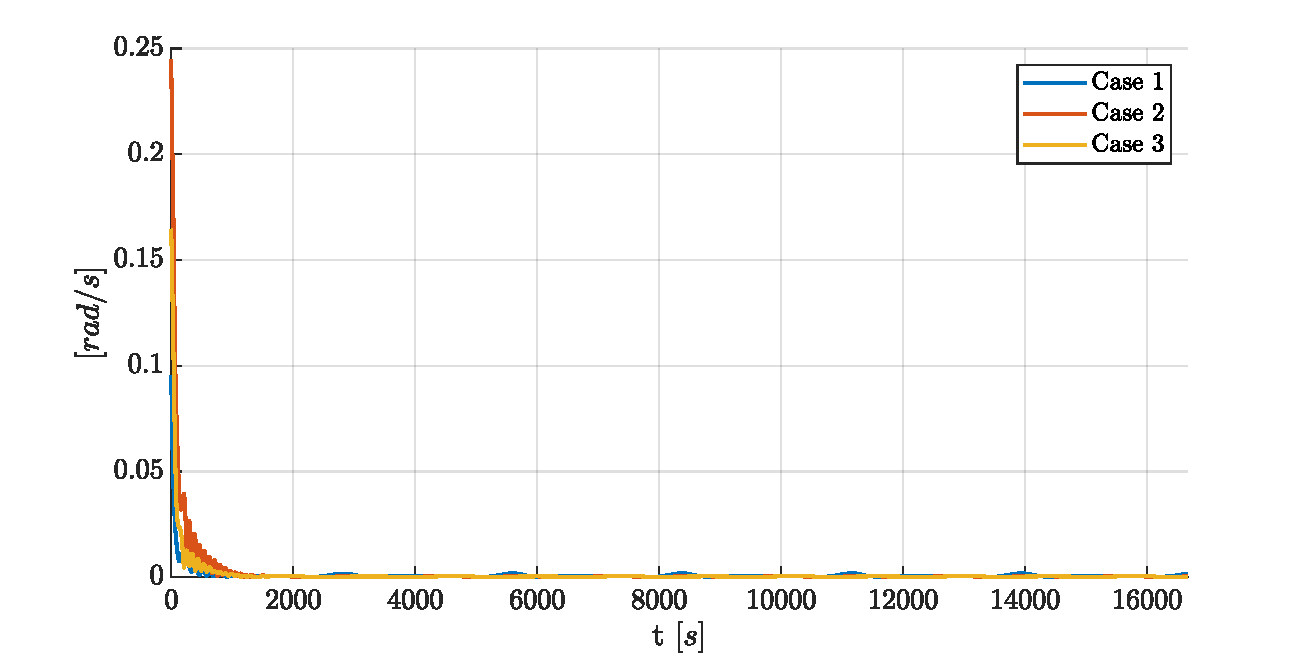
\includegraphics[width=0.8\textwidth]{graphics/offNominal/offNominal-w.pdf}
    \caption{Evolution of $\| \bm{\omega} \|$ (detumbling phase) in the off-nominal cases}
    \label{fig:offNominal-w}
\end{figure}

\begin{figure}[h!]
    \centering
    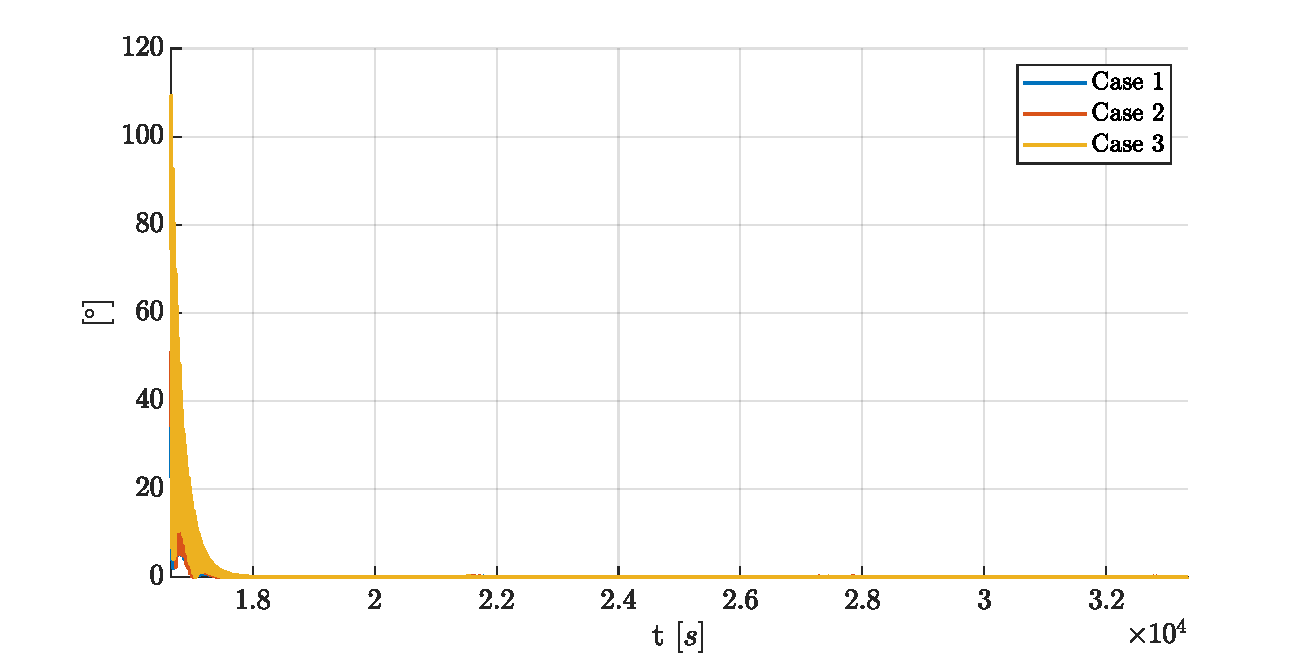
\includegraphics[width=0.8\textwidth]{graphics/offNominal/offNominal-pe.pdf}
    \caption{Evolution of the pointing error (tracking phase) in the off-nominal cases}
    \label{fig:offNominal-pe}
\end{figure}

It is clear that also in these cases the control system satisfies the requirements: the norm of the angular velocity drops to values below $10^{-3} \, rad/s$ in the detumbling phase, while the pointing error is in the order of $10^{-1 \; \circ}$ at the end of the tracking phase. The mission requirements for tracking are therefore still satisfied.

It is important to point out that the expression of the gravity gradient torque used throughout the simulations (\cref{eq:gravity-gradient}) is valid only in the principal axes of inertia, therefore only for diagonal matrices. The presence of the inertia products in the off-nominal conditions is neglected, so the same formula for $\mathbf{M}_{GG}$ is still applied. On the other hand, the disturbances introduced on the control system by the extra-diagonal terms of $I$ (as the control laws are designed on the nominal inertia matrix of the spacecraft) are counteracted through the disturbing torque estimated by the ESO \cite{biggs}.

\section{Conclusions}

The performed numerical simulations indicate that the design of the control system is satisfactory and robust. Detumbling is achieved in both the proposed strategies (though with different degrees of satisfaction) and the pointing error in the tracking phase is kept below the required limit with a sufficiently large margin. A safe margin is very useful as it provides the control system robustness against unmodeled uncertainties. In order to achieve more realistic results, the model of the system shall be improved enhancing some features (for instance, implementing a more complete model for the magnetic field) and including dynamics discarded thus far (as the perturbations for the orbital dynamics).

Future developments to improve the proposed design shall tackle two issues. First, the implementation of a de-saturation mechanism, which is absolutely required in order to extend the mission lifetime. This could be implemented through the already present magnetorquer and a tailored control law. Second, the attitude determination and subsequent estimations shall be improved. This could be done by choosing sensors with faster update rates and by exploiting a different observer.




\clearpage

\printbibliography[heading=bibintoc, title = {References}]

\end{document}
